% =====================================================================================
% PLANTILLA DE TESINA / TESIS  -  Universidad Politécnica de Victoria (UPV)
% Autores: Said Polanco-Martagón, Marco A. Nuño-Maganda   |   Versión reorganizada: ver GUIA_ALUMNO.md
%
% CÓMO USARLA (resumen; los detalles están en GUIA_ALUMNO.md):
%   1. Edita configuracion/datos.tex con tus datos y el tipo de proyecto.
%   2. Escribe cada sección en su archivo de la carpeta secciones/ (lee la «Guía» que trae cada una).
%   3. Agrega tus referencias en referencias/referencias.bib y cítalas con \cite{clave}.
%   4. NO cambies los títulos de las secciones ni borres los comentarios «% audit:req=...»:
%      el sistema de revisión los usa para ubicar cada sección.
% Compilar:  latexmk -pdf main.tex     (usa biber para la bibliografía)
% =====================================================================================

\documentclass[12pt]{article}

% =====================================================================================
% DATOS DEL ALUMNO Y DEL PROYECTO  -->  ESTE ES EL ÚNICO ARCHIVO DE CONFIGURACIÓN QUE DEBES EDITAR
% (además de escribir tus secciones en la carpeta secciones/)
% Cambia solo lo que está entre llaves { } a la derecha de cada \newcommand.
% El sistema de revisión lee estos datos (título, alumno, tipo de proyecto): no cambies los nombres
% de los comandos (\NombreAlumno, \NombreProyecto, \TipoProyecto, ...).
% =====================================================================================

% ---------- Tipo de proyecto (OBLIGATORIO) ------------------------------------------
% Escribe exactamente  sistema   o   investigacion
%   sistema        -> página web, sistema web, API, sistema de escritorio, app móvil
%   investigacion  -> algoritmo, modelo de aprendizaje de máquina u otro trabajo de investigación
% Según el tipo, la Revisión 2 y la 3 piden secciones distintas (ver GUIA_ALUMNO.md).
\newcommand{\TipoProyecto}{sistema}

% ---------- Estilo de citas y referencias -------------------------------------------
% ieee (por defecto) o apa. Pregunta a tu director cuál debes usar.
\newcommand{\EstiloCitas}{ieee}

% ---------- Alumno -------------------------------------------------------------------
\newcommand{\NombreAlumno}{Nombre Apellido Apellido}
\newcommand{\Matricula}{0000000}
% Alumnas: pongan  la  y  a ;  alumnos: pongan  el  y  o
\newcommand{\elolaNombreAlumno}{el}
\newcommand{\OA}{o}

% ---------- Programa y proyecto ------------------------------------------------------
\newcommand{\ncarrera}{Ingeniería en Tecnologías de la Información}
\newcommand{\NombreProyecto}{Título completo del proyecto de estadía}
% Título para el encabezado de cada página. Usa \\ para partirlo en líneas (máximo 3 líneas).
\newcommand{\NombreProyectoheader}{Título completo del proyecto \\de estadía}

% ---------- Organismo receptor (empresa o institución donde realizas la estadía) -----
\newcommand{\organismoreceptor}{Nombre de la empresa o institución}
% Si el organismo es femenino (la universidad, la empresa) pon  la ; si es masculino (el instituto) pon  el
\newcommand{\elolaNombreEmpresa}{la}

% ---------- Asesores y evaluador -----------------------------------------------------
\newcommand{\nasesorinstitucional}{Dr./Dra. Nombre del asesor institucional}
\newcommand{\nasesorempresaria}{Nombre del asesor de la empresa}
\newcommand{\nevalador}{Dr./Dra. Nombre del evaluador}

% ---------- Fechas -------------------------------------------------------------------
\newcommand{\ncuatrimestre}{Mayo-agosto 2026}
\newcommand{\fechaPortada}{Agosto de 2026}
\newcommand{\fechacarta}{1 de Agosto de 2026}
\newcommand{\FechaExposicion}{15 de Agosto de 2026}
\newcommand{\HoraExposionFormatoVenticuatroHoras}{10:00}
       % <-- tus datos (único archivo de configuración que editas)
% =====================================================================================
% PREÁMBULO DE LA PLANTILLA (paquetes y estilos)  -->  NORMALMENTE NO NECESITAS EDITARLO
% Actualización: Said Polanco-Martagón / Marco A. Nuño-Maganda. Reorganizado para el sistema de revisión.
% =====================================================================================

\usepackage[left=2.5cm,top=2.0cm,right=2.5cm,bottom=3.0cm]{geometry}
\usepackage[utf8]{inputenc}
\usepackage[T1]{fontenc}
\usepackage[spanish,mexico]{babel}
\usepackage{etoolbox}
\usepackage{enumitem}                    % listas compactas en las guías
\usepackage[linguistics]{forest}
\usepackage{tikz}
\usepackage{amssymb, amsmath, amsbsy}   % símbolos y ecuaciones
\usepackage{longtable}                  % tablas largas
\usepackage{graphicx}
\usepackage{fancyhdr}
\usepackage{xcolor}
\usepackage{multirow}
\usepackage{listings}
\usepackage{float}                      % necesario para la opción [H] de figuras y tablas
\usepackage{caption}
\usepackage{subcaption}
\usepackage[skip=12pt plus1pt]{parskip}
\usepackage{pdfpages}                   % incluir PDF (cartas) en el documento
\usepackage{verbatim}
\usepackage{algpseudocode}
\usepackage{algorithm}
\usepackage{pdflscape}
\usepackage{afterpage}
\usepackage{array,booktabs,ragged2e}    % booktabs: \toprule \midrule \bottomrule en las tablas
\usepackage{wallpaper}
\usepackage[overload]{textcase}
\usepackage{datetime}

\newcolumntype{L}[1]{>{\raggedright\let\newline\\\arraybackslash\hspace{0pt}}m{#1}}
\newcolumntype{C}[1]{>{\centering\let\newline\\\arraybackslash\hspace{0pt}}m{#1}}
\newcolumntype{R}[1]{>{\raggedleft\let\newline\\\arraybackslash\hspace{0pt}}m{#1}}

\floatname{algorithm}{Algoritmo}
\renewcommand{\listalgorithmname}{Índice de algoritmos}
\renewcommand{\algorithmicrequire}{\textbf{Entrada:}}
\renewcommand{\algorithmicensure}{\textbf{Salida:}}

% ---------------------------------------------------------------------------------------
% REFERENCIAS (biblatex + biber). El estilo se elige en configuracion/datos.tex (\EstiloCitas).
% Archivo de bibliografía: referencias/referencias.bib
% ---------------------------------------------------------------------------------------
\usepackage{csquotes}
\ifdefstring{\EstiloCitas}{apa}
  {\usepackage[backend=biber,style=apa,sorting=nyt]{biblatex}
   \DeclareLanguageMapping{spanish}{spanish-apa}
   % Ajustes adicionales SOLO para el estilo de citas APA (se carga si \EstiloCitas = apa).
% Mejoran el uso de «y» en español y el separador de nombres en la lista de referencias.
\makeatletter
\DefineBibliographyExtras{spanish}{%
  \setcounter{smartand}{1}%
  \let\lbx@finalnamedelim=\lbx@es@smartand
  \let\lbx@finallistdelim=\lbx@es@smartand
}
\makeatother
}
  {\usepackage[backend=biber,style=ieee,sorting=none]{biblatex}}
\addbibresource{referencias/referencias.bib}
\DefineBibliographyStrings{spanish}{references = {Referencias}, bibliography = {Referencias}}

% Permite romper los hipervínculos largos al final de la línea
\setcounter{biburllcpenalty}{7000}
\setcounter{biburlucpenalty}{8000}

\usepackage[bookmarks=true,breaklinks=true,bookmarksopen=false,colorlinks=true,linkcolor=blue]{hyperref}

% Fecha de compilación (se usa en las citas de páginas de Internet)
\newdateformat{specialdate}{\twodigit{\THEDAY}-\twodigit{\THEMONTH}-\THEYEAR}
\date{\specialdate\today}

\newcommand{\HRule}{\rule{\linewidth}{0.25mm}}
\newcommand{\separacionCorta}{0.0cm}
\newcommand{\separacionLarga}{0.5cm}
\newcommand{\iemph}[1]{\MakeTextUppercase{#1}}

% ---------------------------------------------------------------------------------------
% ENCABEZADO Y PIE DE PÁGINA
% ---------------------------------------------------------------------------------------
\pagestyle{fancy}
\setlength{\headheight}{50pt}
\fancyhead{}
\fancyhead[L]{\includegraphics[height=1.00cm]{logos/UTYP.png}}
\fancyhead[C]{\begin{center}\scriptsize{\NombreProyectoheader}\end{center}}
\fancyhead[R]{\includegraphics[height=1.25cm]{logos/LogoUPV_2023.png}}
\fancyfoot{}
\fancyfoot[R]{\thepage}

% ---------------------------------------------------------------------------------------
% GUÍAS PARA EL ALUMNO
% Las guías (entorno guia) explican qué debe ir en cada sección y qué preguntas debe responder.
%   * \guiastrue   -> se muestran en un recuadro (valor inicial, mientras escribes).
%   * \guiasfalse  -> se ocultan en el PDF (cámbialo para la versión final).
% El sistema de revisión IGNORA todo lo que esté dentro de \begin{guia} ... \end{guia}: lo que escribas ahí no
% cuenta como contenido de tu tesina. Escribe tu texto FUERA de las guías.
% ---------------------------------------------------------------------------------------
\usepackage[most]{tcolorbox}
\newif\ifguias
\guiastrue
\newtcolorbox{guiabox}[1][]{breakable, enhanced jigsaw, colback=yellow!10, colframe=orange!70!black,
  fonttitle=\bfseries\small, title={#1}, boxrule=0.6pt, arc=2pt, left=5pt, right=5pt, top=3pt, bottom=3pt,
  fontupper=\small, before skip=8pt, after skip=10pt}
\newenvironment{guia}[1][Guía para el alumno]
  {\ifguias\begin{guiabox}[#1]\else\setbox0\vbox\bgroup\fi}
  {\ifguias\end{guiabox}\else\egroup\fi}
   % paquetes, estilos y guías (no editar)

\begin{document}

%-----------------------------------------------------------------------------------------------------------------
% PARTES INSTITUCIONALES (portada, cartas y evaluación). Se generan con tus datos; no las edites.
%-----------------------------------------------------------------------------------------------------------------
%-----------------------------------------------------------------------------------------------------------------
% PAGINA 1 - PORTADA
\setcounter{page}{1}
\pagenumbering{roman}
\thispagestyle{empty}

\begin{center}

\begin{tabular}{cp{5cm}c}
\includegraphics[height=2.25cm]{logos/UTYP.png} & 
& \includegraphics[height=2.25cm]{logos/LogoUPV_2023.png}   \\
\end{tabular}

\Large \textbf{UNIVERSIDAD POLITÉCNICA DE VICTORIA}
\vspace{0.5cm}
\hrule
\vspace{0.1cm} 
\hrule
\vspace{0.5cm}


%\HRule \\[\separacionCorta]
\textbf{\iemph{\NombreProyecto}} \\[\separacionLarga]
%\Large \textbf{TESINA}
%\HRule \\[\separacionLarga]
T E S I N A \\
QUE PARA OBTENER EL GRADO DE \\
\textbf{\iemph{\ncarrera}} \\[\separacionLarga]

PRESENTA: \\[\separacionCorta]
%\textbf{\Capitalize{\NombreAlumno}\\[\separacionLarga]
\textbf{\iemph{\NombreAlumno}}\\[\separacionLarga]
%EN CUMPLIMIENTO DE \\[\separacionCorta]
%LA ESTADÍA DE LA CARRERA DE \\[\separacionCorta]


DIRECTOR \\[\separacionCorta]
\textbf{\iemph{\nasesorinstitucional}} \\[\separacionCorta]

CO-DIRECTOR \\[\separacionCorta]
\textbf{\iemph{\nasesorempresaria}} \\[\separacionCorta]

ORGANISMO RECEPTOR \\[\separacionCorta]
\textbf{\iemph{\organismoreceptor}} \\[\separacionLarga]

\end{center}
\begin{flushright}
\iemph{Ciudad Victoria, Tamaulipas, \fechaPortada}
\end{flushright}

\HRule 



% En las siguientes 3 paginas, debe incluir una digitalización de calidad de sus respectivas cartaas, no una fotografia toda cucha tomada con su celular de Coppel
% Pagina 1: Digitalización de la carta de presentación (sustituir por una original en el empastado)
\clearpage
\thispagestyle{fancy}
\pagenumbering{roman}
\setcounter{page}{1}
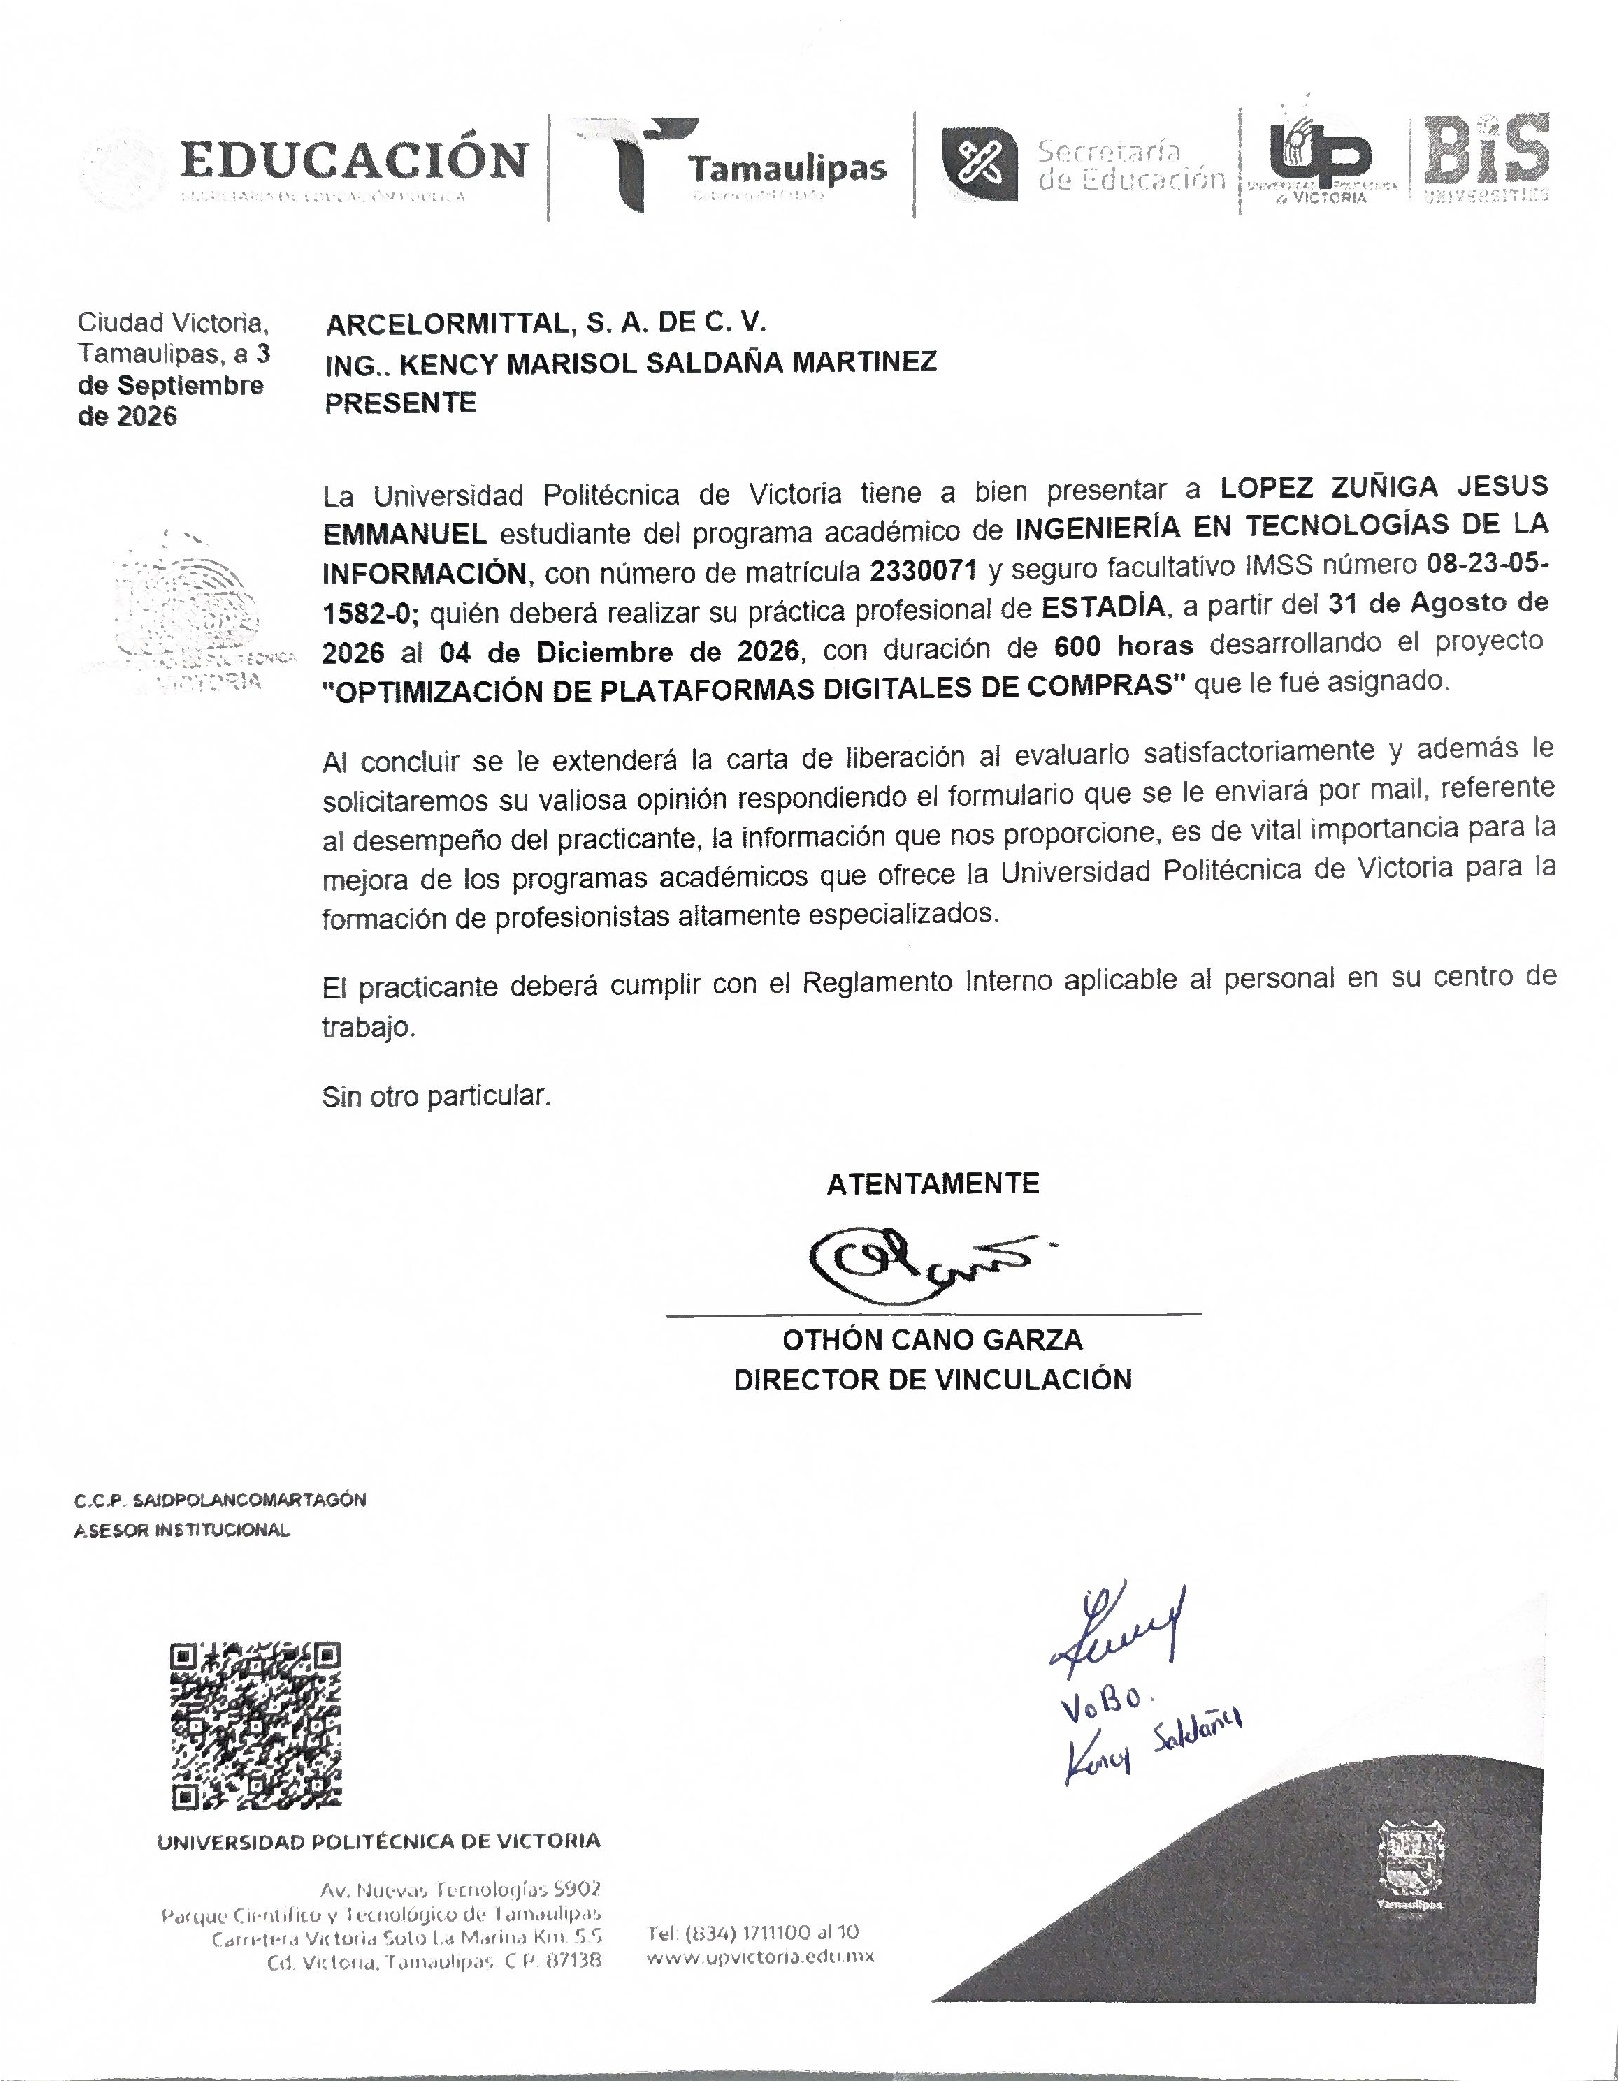
\includepdf[pages={1}]{cartas/CartaPresentacion.pdf}

% Pagina 2: Digitalización de la carta de aceptación (sustituir por una original en el empastado)
\clearpage
\thispagestyle{fancy}
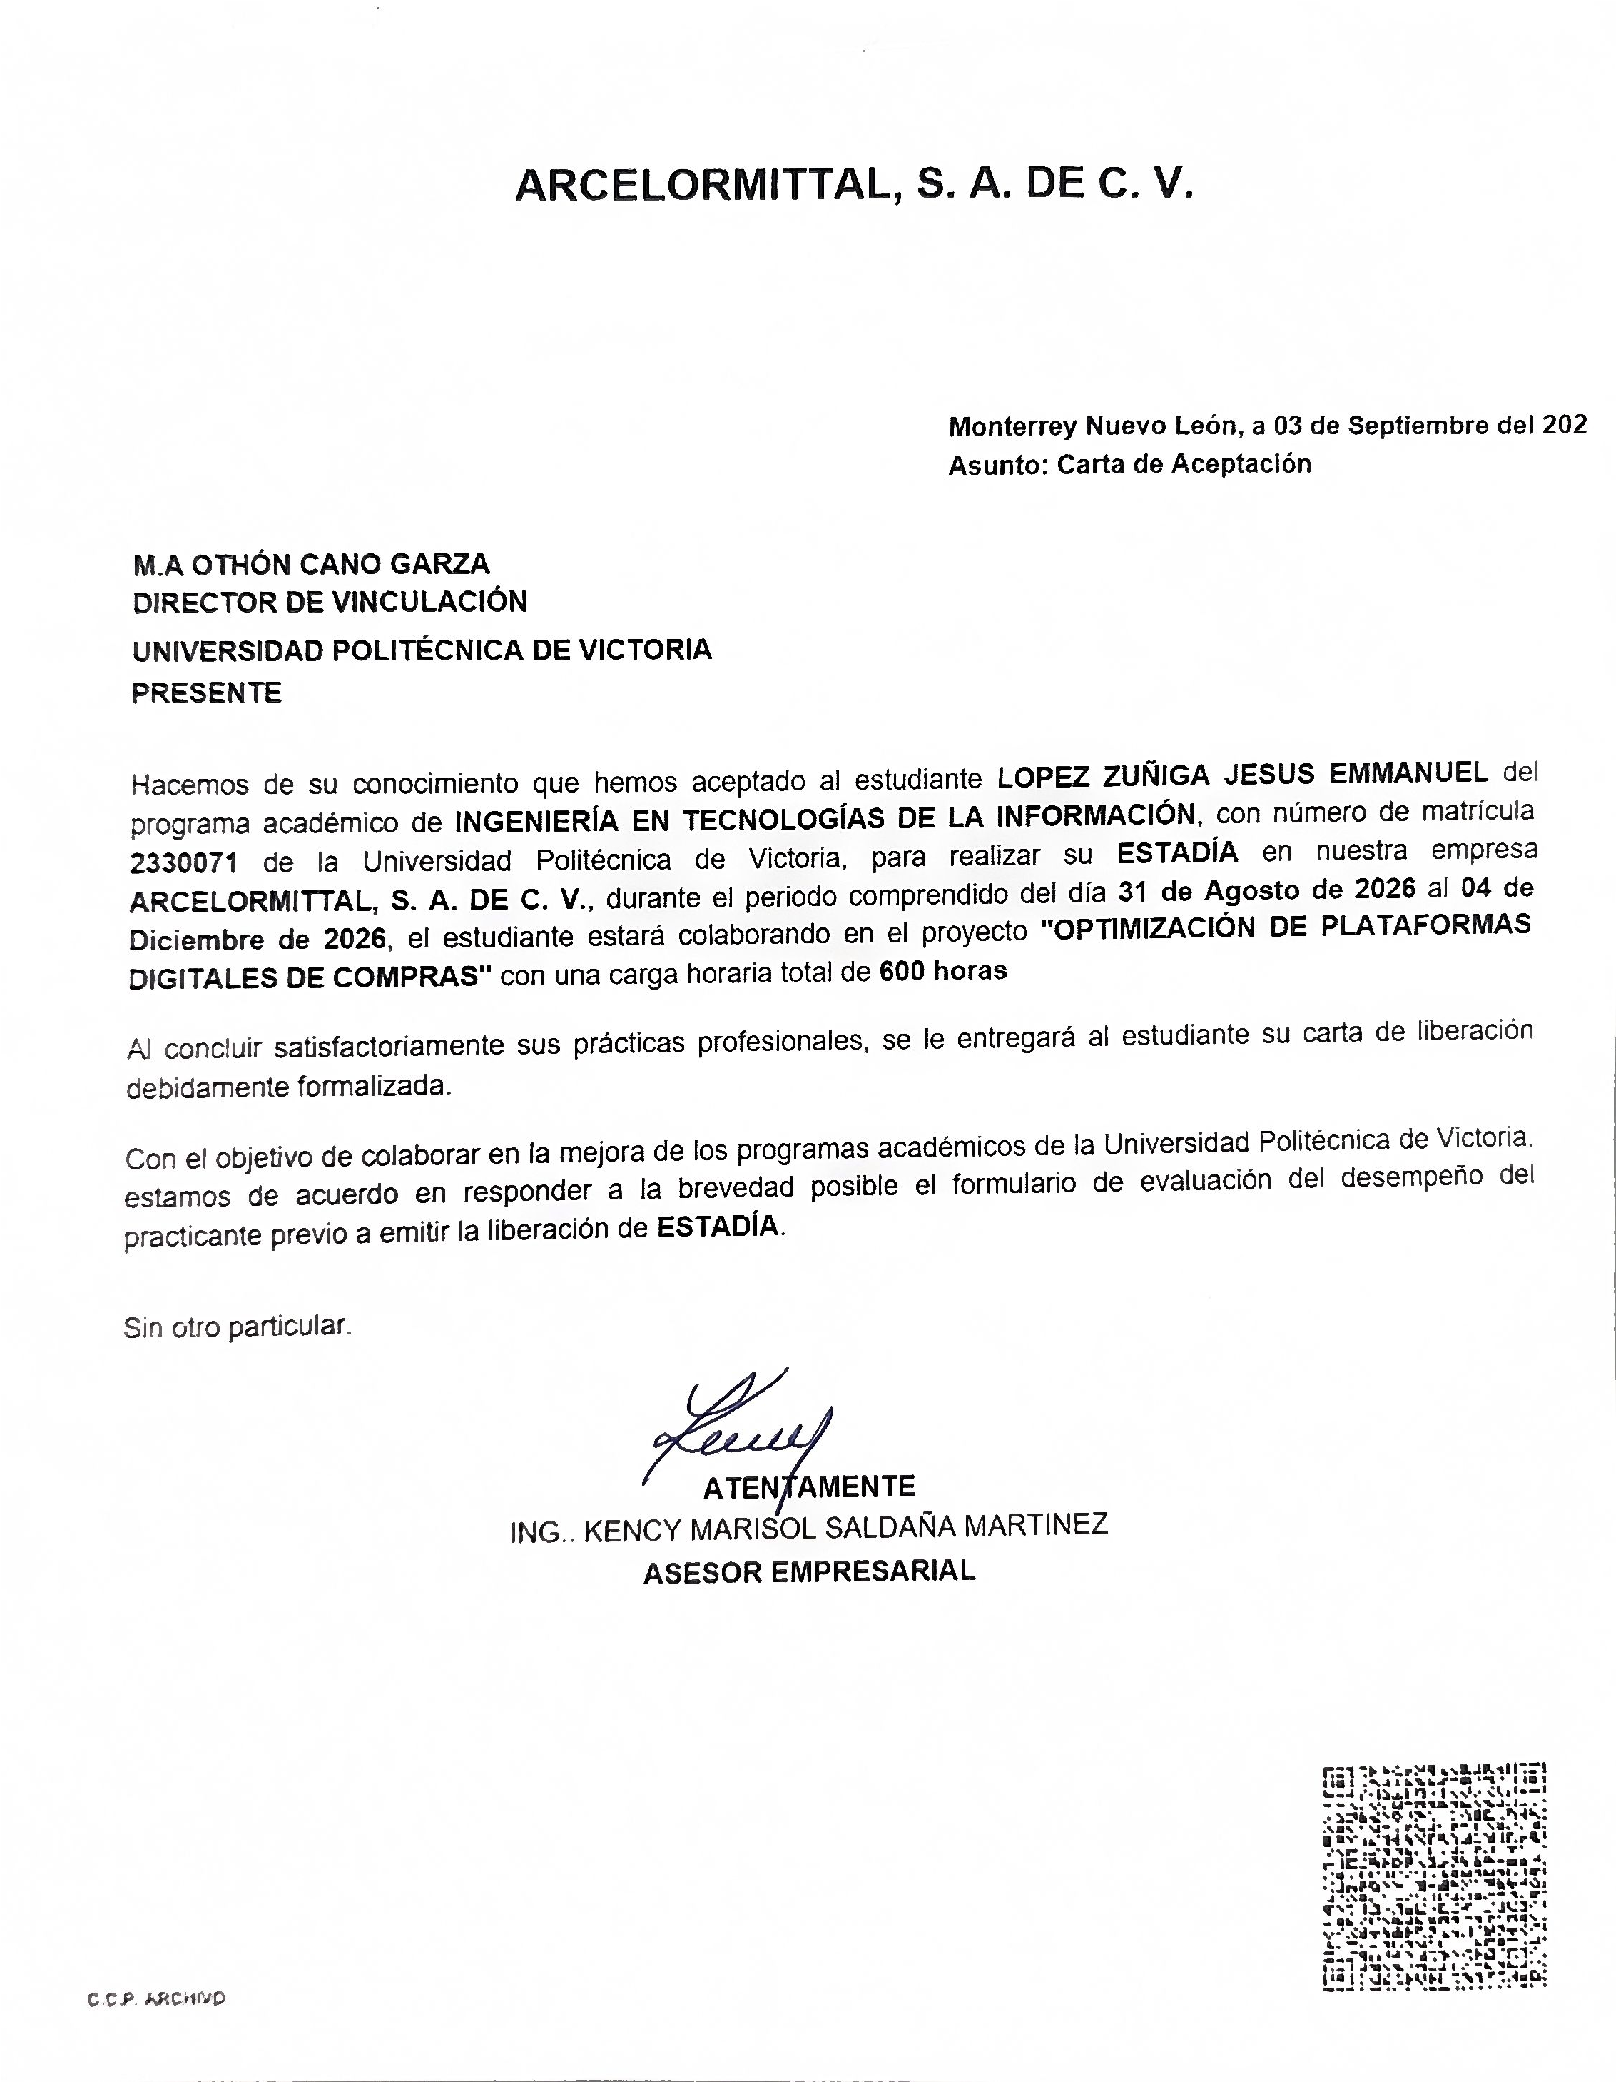
\includepdf[pages={1}]{cartas/CartaAceptacion.pdf}

% Pagina 3: Digitalización de la carta de liberación (sustituir por una original en el empastado)
\clearpage
\thispagestyle{fancy}
\includepdf[pages={1}]{cartas/CartaLiberacion.pdf}

% Pagina 4: Carta de aceptación del ASESOR INSTITUCIONAL(sustituir por una original en el empastado)
\clearpage
\ULCornerWallPaper{1}{membretes/membrete_UPV_08May25.pdf}
\thispagestyle{empty}

\vspace*{1.5cm}
\large

\begin{center}
\textbf{CARTA DE ACEPTACIÓN DEL DOCUMENTO PARA SU IMPRESIÓN}\\[\separacionLarga]
\end{center}

\begin{flushright}
Cd. Victoria, Tamaulipas a \fechacarta \\[\separacionLarga]
\end{flushright}

\parindent=0mm

\NombreAlumno \\
PRESENTE \\[\separacionCorta]

Le comunico que  el Programa Académico de \ncarrera\ \ le ha otorgado la autorización para la impresión de su Tesina de Estadía Práctica cuyo título es: \\[\separacionCorta]

\begin{center}
\textbf{\NombreProyecto} \\[\separacionLarga]
\end{center}

\begin{center}	
\begin{tabular}{ccc}
\centering
& ATENTAMENTE & \\ 
& & \\
& & \\
& & \\ \hline
& \nasesorinstitucional & \\
& ASESOR INSTITUCIONAL & \\
\end{tabular}
\end{center} 
\vspace{2cm}
c.c.p Director de programa académico

            % antes de imprimir: sustituye los PDF de cartas/ por tus cartas escaneadas
%-----------------------------------------------------------------------------------------------------------------
\clearpage
\ClearWallPaper
\thispagestyle{empty}
\newgeometry{left=1.5cm,top=1.0cm,right=1.5cm,bottom=2.0cm}             
\begin{landscape}

%\afterpage{\restoregeometry}


\begin{tabular}{p{3cm}p{16cm}p{3cm}}
\multirow{4}{*}{\includegraphics[width=3.0cm]{logos/UTYP.png}} &  & \multirow{4}{*}{\includegraphics[width=3.0cm]{logos/LogoUPV_2023.png}} \\
   & \multicolumn{1}{c}{\textbf{EVALUACIÓN DE ESTADÍA}} &  \\ %\cline{2-2}
& \multicolumn{1}{c}{\textbf{Rúbrica para evaluación de la presentación y el reporte de estadía}} & \\ 
& & \\ 
\end{tabular}

\normalsize
\begin{tabular}{p{13cm}R{10cm}}
\multicolumn{1}{l}{Nombre del alumno: \underline{\textbf{\iemph{\NombreAlumno}}}}  & 
Calificación final: \underline{\hspace{3cm}}    \\ %\cline{2-2}
\multicolumn{2}{c}{Periodo: \underline{\textbf{\iemph{\ncuatrimestre}}}}    \\ %\cline{2-2}
& \\
\end{tabular}

\scriptsize 
%\begin{center}
%\resizebox{\linewidth}{!}{%
\begin{tabular}{C{2.0cm}|C{2.0cm}|C{4.5cm}|C{4.5cm}|C{4.5cm}|C{4.5cm}}
\hline
\multirow{2}{*}{Ponderación} & Aspecto a  & Competente & Independiente & Básico Avanzado & No Competente \\
 & Evaluar & 10 & 9 & 8 & 5 \\ 
\hline
40 & Resultados y Actividades & Estrechamente relacionados al perfil de
egreso de su programa académico & Parcialmente relacionados al perfil de
egreso de su programa académico & Escasamente relacionados al perfil de egreso de su programa académico & Escasamente relacionados al perfil de egreso de su programa académico \\  \hline

30 & Exposición de las actividades de la estadía  & Detalladas y sustentadas con respecto a los resultados que se obtuvieron & Detalladas y sustentadas parcialmente con respecto a los resultados que se obtuvieron & Detalladas parcialmente con respecto a los resultados que se obtuvieron & Detalladas escazamente con respecto a los resultados que se obtuvieron \\  \hline 

10 & Material visual Lenguaje
verbal & Uso el lenguaje y la terminología
apropiadas; El material visual está organizado,
adecuado y suficiente
 & 
Uso el lenguaje y la terminología apropiadas
El material visual está parcialmente
organizado y es suficiente
& 
Uso el lenguaje y la terminología son parcialmente apropiadas; El material visual está parcialmente
organizado y es suficiente
 & 
Uso el lenguaje y terminología es inapropiado; El material visual no está organizado y es insuficiente
 \\  \hline
10 & Exposición en Idioma Inglés &

Pronunciation is clear so language is easily understood (2.5) Uses fluent connected speech, occasionally disrupted by search for correct form of expression (2.5) Uses topic related vocabulary without problems (2.5) Responds to questions using varied and descriptive vocabulary and language structures (2.5) & 

Pronunciation is understandable, but there are slight errors (2.25)
Speech is connected but frequently disrupted by search for correct form of
expression (2.25) Uses some topic related vocabulary sufficient to communicate ideas (2.25) Responds to questions using simple but accurate vocabulary and language structures (2.25 & 

Pronunciation is understandable most of the time, marked native accent and many errors
(2) Speaks with simple sentences, sometimes not connected, but is understood (2) Uses basic vocabulary to communicate ideas
(2) Partly responds to simple questions, with limited vocabulary and language structures (2)  &

Pronunciation makes language very difficult to understand (1) Uses one-word/two-word utterances (1) Unable to communicate ideas due to lack of vocabulary (1) Uses isolated words or sentence fragments to respond to questions (1) 
\\  \hline

5 & Respuesta a los cuestionamientos de los evaluadores & 
Clara y satisfactoria & 
Clara y parcialmente satisfactoria & 
Clara e insuficiente & 
Confusa e insuficiente 
\\  \hline
5 & Autorización de tesina en tiempo y forma & 
Presenta en tiempo y forma 
\tikz[overlay, remember picture,anchor=base]  \node (Mark){}; 
 & 
Presenta en tiempo y forma con la mayoría de requerimientos solicitados & 
Presenta en tiempo y con algunas limitantes  de los requerimientos solicitados. &
Presenta fuera de tiempo y con los mínimos requerimientos solicitados.
 \\  % Una linea en Blanco para poner la marca del ASESOR INSTITUCIONAL
&
&
%\tikz[overlay, remember picture,anchor=base] \node (Center){};

&
 \\  \hline

\end{tabular}

%\begin{tikzpicture}[remember picture, overlay, note/.style={rectangle callout, fill=#1}]
%\node [note=red!80, callout absolute pointer={(Mark)}] at (Center) {COMPETENTE!};
%\end{tikzpicture}

%}
%\end{center}

\normalsize


%\begin{center}
%\begin{tabular}{ccc}
%\includegraphics[scale=0.10]{FirmaMANM2.png} & & \\
%\hline 
%\nasesorinstitucional & \nevalador & \\
%ASESOR INSTITUCIONAL & EVALUADOR & EVALUADOR INGLÉS \\
%\end{tabular}
%\end{center}

\begin{center}
\begin{tabular}{cp{1cm}cp{1cm}c}
%\includegraphics[scale=0.10]{ArchivoFirmaASESOR.png} & & & & \\
 & & & & \\
  & & & & \\
\hline 
\nasesorinstitucional & & \nevalador & & \\
ASESOR INSTITUCIONAL & &EVALUADOR & &EVALUADOR DE INGLÉS \\
\end{tabular}
\end{center}


\end{landscape} 
\restoregeometry

%-----------------------------------------------------------------------------------------------------------------
% Pagina 5: Registro de Evaluación de Estadía
\clearpage
\pagestyle{empty}
\ULCornerWallPaper{1}{membretes/membrete_UPV_08May25.pdf}

\vspace*{0.5cm}



\large
\begin{center}
\textbf{REGISTRO DE EVALUACIÓN DE EXPOSICIÓN DE ESTADÍA}
\\[\separacionLarga]
\end{center}


Siendo las \HoraExposionFormatoVenticuatroHoras \ \ horas del día \FechaExposicion, \elolaNombreAlumno\ \ alumn\OA\ \ \textbf{\NombreAlumno}, del programa académico \textbf{\ncarrera}, con matricula \textbf{\Matricula}, presentó la exposición de la estadía realizada durante el cuatrimestre \textbf{\ncuatrimestre}, en \elolaNombreEmpresa\ \ \textbf{\organismoreceptor}, con el proyecto titulado \textbf{\NombreProyecto}.\\

Una vez concluido el proceso de evaluación, y con base a la rúbrica establecida para éste propósito, se determina que la calificación de la estadía es \underline{\hspace{2cm}}. %\hrulefill.

\begin{center}
\begin{tabular}{ccc}
& & \\
& & \\
& & \\
%& \includegraphics[scale=0.10]{FirmaAsesorPro.png} & \\
\hline 
%& \underline{\hspace{8cm}}& \\
& \nasesorinstitucional & \\
& ASESOR INSTITUCIONAL & \\
& & \\
& & \\
& & \\
%& \underline{\hspace{8cm}}& \\
\hline 
& \nevalador & \\
& EVALUADOR & \\
& & \\
& & \\
%& & \\
\hline 
& & \\
& EVALUADOR DE INGLÉS & \\
\end{tabular}
\end{center}

\normalsize


%-----------------------------------------------------------------------------------------------------------------
% AGRADECIMIENTOS, RESUMEN, SUMMARY E ÍNDICE
%-----------------------------------------------------------------------------------------------------------------
% =====================================================================================
% AGRADECIMIENTOS, RESUMEN (Revisión 4) Y SUMMARY
% Escribe tu texto FUERA de los recuadros \begin{guia} ... \end{guia}.
% =====================================================================================

\clearpage
\ClearWallPaper
\pagestyle{fancy}

\section*{\centering Agradecimientos}
\addcontentsline{toc}{section}{Agradecimientos}
% >>> ESCRIBE AQUÍ tus agradecimientos (opcional, breve) <<<


\clearpage
\section*{\centering Resumen} % audit:req=resumen
\addcontentsline{toc}{section}{Resumen}

\begin{guia}[Guía: Resumen (Revisión 4)]
\textbf{¿Para qué sirve?} Es la síntesis de todo el trabajo para quien no leerá el documento completo. Se escribe al
final, cuando ya tienes los resultados.

\textbf{Debe responder, en un solo párrafo de 150 a 250 palabras:} ¿cuál es el contexto y el problema? ¿cuál es el
objetivo? ¿qué se hizo (método o solución)? ¿cuáles fueron los resultados principales (con datos)? ¿cuál es la
conclusión o aportación?

\textbf{Reglas:} sin citas, sin figuras, sin siglas sin definir. Cierra con \textbf{4 a 6 palabras clave} (en
minúsculas, separadas por comas).

\textbf{Extensión mínima:} 120 palabras.
\end{guia}

% >>> ESCRIBE AQUÍ el resumen (un párrafo) <<<

\textbf{Palabras clave:} palabra1, palabra2, palabra3, palabra4.


\clearpage
\section*{\centering Summary}
\addcontentsline{toc}{section}{Summary}

\begin{guia}[Guía: Summary (Revisión 4)]
Traducción al inglés del Resumen (mismo contenido y estructura), con \textbf{Keywords}. Revisa la gramática; evita
traducción automática literal.
\end{guia}

% >>> WRITE HERE the English summary <<<

\textbf{Keywords:} keyword1, keyword2, keyword3, keyword4.
       % Agradecimientos, Resumen, Summary         [Revisión 4]

\clearpage
\addcontentsline{toc}{section}{Índice}
\renewcommand\contentsname{Índice}
\tableofcontents

%-----------------------------------------------------------------------------------------------------------------
% CUERPO DEL DOCUMENTO. Cada revisión agrega secciones; puedes ir llenándolas en orden.
%-----------------------------------------------------------------------------------------------------------------
\clearpage
\pagenumbering{arabic}
\setcounter{page}{1}

% ---- Revisión 1 ---------------------------------------------------------------------------------
% =====================================================================================
% REVISIÓN 1  -  Introducción, Planteamiento del problema, Objetivos, Justificación, Alcances y limitaciones
% Escribe tu texto FUERA de los recuadros \begin{guia} ... \end{guia}.
% No cambies los títulos ni borres los comentarios «% audit:req=...» al final de cada \section / \subsection.
% =====================================================================================

\section{Introducción} \label{sec:introduccion} % audit:req=introduccion

\begin{guia}[Guía: Introducción (Revisión 1)]
\textbf{¿Para qué sirve?} Presenta tu trabajo a un lector que no lo conoce y lo invita a seguir leyendo. Es el resumen
``de entrada'' del proyecto: contexto, problema, propuesta y organización del documento.

\textbf{Debe responder:}
\begin{itemize}[nosep,leftmargin=*]
  \item ¿En qué contexto (sector, empresa, área tecnológica) se desarrolla el proyecto?
  \item ¿Cuál es el problema o la necesidad, dicho en pocas líneas? (el detalle va en \emph{Planteamiento del problema}).
  \item ¿Qué se propone hacer y qué se espera lograr?
  \item ¿Por qué es importante? (una idea; el detalle va en \emph{Justificación}).
  \item ¿Cómo está organizado el documento? (una frase por sección o capítulo).
\end{itemize}

\textbf{Extensión mínima:} 150 palabras (1 a 2 páginas), redactadas con tus propias palabras.

\textbf{Errores frecuentes:} copiar definiciones de Internet; escribir solo ``en este capítulo se verá\ldots'' sin decir
nada concreto; dejar la introducción para el final y no actualizarla cuando el proyecto cambia.

\textbf{Cómo se revisa:} claridad del contexto, que el problema y la propuesta se entiendan sin leer el resto, y que la
organización descrita coincida con las secciones reales del documento.
\end{guia}

% >>> ESCRIBE AQUÍ el texto de la introducción (fuera de la guía) <<<


\subsection{Planteamiento del problema} \label{sec:problema} % audit:req=planteamiento

\begin{guia}[Guía: Planteamiento del problema (Revisión 1)]
\textbf{¿Para qué sirve?} Describe con precisión la situación que quieres resolver y demuestra que es un problema real.

\textbf{Debe responder:}
\begin{itemize}[nosep,leftmargin=*]
  \item ¿Qué situación actual es insatisfactoria o genera una necesidad? Descríbela con hechos, ejemplos o cifras.
  \item ¿Quién la padece (usuarios, área, empresa) y cómo se manifiesta (retrasos, errores, costos, quejas)?
  \item ¿Qué consecuencias tiene no resolverla?
  \item ¿Qué se ha intentado hasta ahora y qué falta (la brecha)? Conecta con los \emph{Antecedentes}.
  \item ¿Cuál es el problema en una sola frase? Escríbelo como enunciado del problema o como pregunta de
        investigación (p. ej. ``¿Cómo reducir X en Y mediante Z?'').
\end{itemize}

\textbf{Extensión mínima:} 120 palabras.

\textbf{Errores frecuentes:} describir la solución en lugar del problema (``el problema es que no hay un sistema web'');
problemas sin evidencia; enunciados tan amplios que no se pueden resolver en una estadía.

\textbf{Cómo se revisa:} que el problema esté delimitado, sea verificable y que los objetivos lo atiendan.
\end{guia}

% >>> ESCRIBE AQUÍ el planteamiento del problema <<<


\subsection{Objetivos} \label{sec:objetivos} % audit:req=objetivos

\begin{guia}[Guía: Objetivo general y objetivos específicos (Revisión 1)]
\textbf{¿Para qué sirve?} Fija qué vas a lograr. Todo lo demás (resultados y conclusiones) se compara contra estos objetivos.

\textbf{Objetivo general} (uno): verbo en infinitivo + qué se hará + con qué o cómo + para qué, y si es posible un criterio
medible. \emph{Ejemplo:} ``Desarrollar un sistema web de notificaciones para familiares de pacientes hospitalizados que
reduzca en 50\% las llamadas de consulta al área de enfermería.''

\textbf{Objetivos específicos} (de 3 a 6): pasos concretos y verificables que, al cumplirse, logran el objetivo general.
Cada uno debe poder demostrarse con un resultado (un módulo, un diagrama, un experimento) que luego aparecerá en
\emph{Resultados} y se retomará en \emph{Conclusiones}. Deben ser SMART: específicos, medibles, alcanzables, relevantes y
con tiempo definido.

\textbf{Debe responder:} ¿qué voy a entregar? ¿cómo sabré que lo logré? ¿cada objetivo específico aporta al general?

\textbf{Extensión mínima:} 40 palabras en total.

\textbf{Errores frecuentes:} verbos no medibles (``conocer'', ``entender'', ``estudiar''); objetivos que son actividades
(``investigar sobre\ldots'') y no logros; más de un objetivo general; objetivos que luego no se atienden en el documento.

\textbf{Cómo se revisa:} coherencia con el problema, medibilidad y que cada objetivo tenga un resultado asociado.
\end{guia}

\subsubsection{Objetivo general} \label{subsec:objetivo_general}
% >>> ESCRIBE AQUÍ el objetivo general (una sola oración) <<<

\subsubsection{Objetivos específicos} \label{subsec:objetivos_especificos}
% >>> ESCRIBE AQUÍ los objetivos específicos como lista numerada: \begin{enumerate} \item ... \end{enumerate} <<<


\subsection{Justificación} \label{sec:justificacion} % audit:req=justificacion

\begin{guia}[Guía: Justificación (Revisión 1)]
\textbf{¿Para qué sirve?} Explica por qué vale la pena dedicar tiempo y recursos a este proyecto.

\textbf{Debe responder:}
\begin{itemize}[nosep,leftmargin=*]
  \item ¿Quién se beneficia y de qué manera? (empresa, usuarios, la comunidad, tú).
  \item ¿Qué se gana en términos prácticos, económicos, sociales, tecnológicos o científicos? Usa datos cuando existan.
  \item ¿Qué pasaría si no se hace?
  \item ¿Por qué es viable hacerlo ahora y por qué con este enfoque?
  \item ¿Cómo se relaciona con el perfil de egreso de tu programa académico?
\end{itemize}

\textbf{Extensión mínima:} 100 palabras.

\textbf{Errores frecuentes:} repetir el problema con otras palabras; afirmaciones sin sustento (``mejorará mucho la
eficiencia''); olvidar al beneficiario.

\textbf{Cómo se revisa:} que los beneficios sean concretos y consistentes con el problema y los objetivos.
\end{guia}

% >>> ESCRIBE AQUÍ la justificación <<<


\subsection{Alcances y limitaciones} \label{sec:alcances_limitaciones} % audit:req=alcances

\begin{guia}[Guía: Alcances y limitaciones (Revisión 1)]
\textbf{¿Para qué sirve?} Marca las fronteras del proyecto para evitar expectativas irreales.

\textbf{Alcances} -- lo que \emph{sí} incluye el trabajo. Debe responder: ¿qué módulos, funciones, procesos, usuarios o
datos se cubren? ¿en qué plataformas o entornos? ¿qué entregables habrá? ¿qué queda \emph{explícitamente fuera}?

\textbf{Limitaciones} -- lo que restringe el trabajo y que no depende totalmente de ti. Debe responder: ¿qué límites hay
de tiempo (un cuatrimestre), recursos, acceso a datos o a la infraestructura de la empresa, tecnología, permisos?
¿cómo pueden afectar la validez o generalización de los resultados?

\textbf{Extensión mínima:} 60 palabras en total.

\textbf{Errores frecuentes:} prometer más de lo que cabe en la estadía; confundir limitaciones con excusas; no decir qué
queda fuera.

\textbf{Cómo se revisa:} realismo del alcance y honestidad de las limitaciones.
\end{guia}

\subsubsection{Alcances} \label{subsec:alcances}
% >>> ESCRIBE AQUÍ los alcances <<<

\subsubsection{Limitaciones} \label{subsec:limitaciones}
% >>> ESCRIBE AQUÍ las limitaciones <<<
       % Introducción, Planteamiento, Objetivos, Justificación, Alcances y limitaciones
\clearpage
% =====================================================================================
% REVISIÓN 1  -  Antecedentes (del problema, de la empresa y teóricos) y tabla comparativa
% Escribe tu texto FUERA de los recuadros \begin{guia} ... \end{guia}.
% =====================================================================================

\section{Antecedentes} \label{sec:antecedentes}

Este capítulo sitúa el proyecto en tres planos. Primero, los antecedentes del problema: cómo se atendía antes la necesidad y qué trabajos existen sobre ella. Después, la empresa y el proceso donde se desarrolla. Por último, los conceptos y tecnologías que lo sustentan, junto con una tabla comparativa de trabajos relacionados.

\begin{guia}[Guía: Antecedentes (Revisión 1)]
Este capítulo sitúa tu proyecto: qué se ha hecho antes, en qué organización ocurre y qué conceptos lo sustentan.
Tiene tres apartados (\emph{del problema}, \emph{de la empresa}, \emph{teóricos}) y una \emph{tabla comparativa}.
Escribe aquí, si quieres, un párrafo breve que presente los apartados.
\end{guia}

\subsection{Antecedentes del problema} \label{sec:antecedentes_problema} % audit:req=antecedentes

\begin{guia}[Guía: Antecedentes del problema (Revisión 1)]
\textbf{¿Para qué sirve?} Muestra que conoces lo que ya existe sobre el problema y justifica que haga falta tu trabajo.

\textbf{Debe responder:}
\begin{itemize}[nosep,leftmargin=*]
  \item ¿Cómo ha evolucionado o se ha enfrentado este problema? (breve recorrido histórico o de contexto).
  \item ¿Qué soluciones, sistemas, tesis o artículos existentes abordan el mismo problema o uno parecido (mínimo 3, con
        cita \verb|\cite{clave}|)?
  \item ¿Qué hace cada uno, qué ventajas y qué limitaciones tiene?
  \item ¿Qué queda sin resolver y cómo se conecta con tu propuesta?
\end{itemize}

\textbf{Extensión mínima:} 120 palabras. \textbf{Fuentes:} libros, artículos, documentación técnica oficial o sistemas
reales; evita depender solo de blogs.

\textbf{Errores frecuentes:} listar herramientas sin analizarlas; no citar; copiar descripciones comerciales.

\textbf{Cómo se revisa:} pertinencia de las fuentes, análisis crítico y conexión explícita con el problema.
\end{guia}

% >>> ESCRIBE AQUÍ los antecedentes del problema <<<

Antes de este proyecto, el control de compras y de proveedores se apoyaba en los registros nativos de SAP e IMaS, sin un mecanismo automatizado que cruzara la información entre ambos.
Al asumir la responsabilidad del proyecto, la aplicación RM-Inventory ya estaba desarrollada sobre Power Platform con una separación de responsabilidades: archivos de Excel con Office Scripts realizaban el proceso ETL, Power Automate orquestaba los procesos, las listas de SharePoint funcionaban como modelo de datos operativo, Power Apps era la interfaz de usuario y Power BI la capa analítica. Sin embargo, presentaba fallas lógicas y de diseño. El archivo Excel maestro debía actualizarse manualmente cada día para poder consultarlo desde Power Apps. El módulo de inicio de sesión y gestión de usuarios podía eliminarse, porque el control de acceso se resuelve con los permisos del propio entorno. La pantalla de inicio mostraba contenedores provisionales que debían sustituirse por un tablero de Power BI embebido a pantalla completa. De los módulos construidos, solo Arrivals y Consumption tenían pruebas funcionales completas; el proceso ETL y el envío de alertas por correo operaban de forma estable, pero el segundo se ejecutaba manualmente y faltaba configurar un desencadenador programable.
En paralelo existía el desarrollo del proyecto INDICADORES, una plantilla de Excel donde cada fila se completaba manualmente con la información que los datos de origen no contenían, y que Power BI replicaba para aplicar filtros y operaciones, incluida una gráfica de la evolución del precio por material. Faltaba migrarlo a una interfaz en Power Apps que reprodujera la plantilla, incorporara nuevos apartados de registro, embebiera el tablero y resolviera el manejo de históricos y de información de proveedores.
Fuera de la empresa, trabajos recientes abordan problemas parecidos con herramientas similares (Tabla~\ref{tab:comparativa_antecedentes}). Rojas y Hernández \cite{rojas2025rpaessa} automatizaron con Python, Power Automate y Power BI el seguimiento analítico de activos, y reportan una reducción de 38 a 3.33 horas mensuales. Galeano \cite{galeano2025} automatizó con Power Apps, Power Automate y Python tareas de facturación, impuestos y activos fijos, aunque su resumen no incluye cifras de resultados. Osorio \cite{osorio2026} logró la interoperabilidad entre Excel y un ERP para reducir cruces manuales y reprocesos en pedidos e inventario, con un tiempo promedio reportado de 19 minutos. Monroy \cite{monroy2025} construyó un tablero en Power BI con datos centralizados, validado funcionalmente. Ninguno combina en una sola solución la conciliación entre SAP e IMaS, el seguimiento del inventario de materias primas junto con las órdenes de compra activas y la automatización de los flujos que lo alimentan, que es la brecha que este proyecto atiende.

\subsection{Antecedentes de la empresa} \label{sec:antecedentes_empresa} % audit:req=antecedentes_empresa

\begin{guia}[Guía: Antecedentes de la empresa u organismo receptor (Revisión 1)]
\textbf{¿Para qué sirve?} Describe la organización donde realizas la estadía y el proceso que tu proyecto mejora.

\textbf{Debe responder:}
\begin{itemize}[nosep,leftmargin=*]
  \item ¿Quién es el organismo receptor? (giro o sector, ubicación, breve historia, misión y visión).
  \item ¿Cuál es su estructura y en qué área o departamento se realiza tu proyecto? (organigrama opcional).
  \item ¿Cómo se realiza hoy el proceso que vas a mejorar? ¿con qué personas, herramientas o sistemas?
  \item ¿Quién es tu asesor empresarial y cuál es su función?
\end{itemize}

\textbf{Extensión mínima:} 100 palabras.

\textbf{Cuidado:} pide autorización a la empresa para publicar información; no incluyas datos confidenciales ni
datos personales.

\textbf{Errores frecuentes:} copiar la página web de la empresa; no describir el proceso actual (es lo más importante).

\textbf{Cómo se revisa:} que se entienda el contexto operativo real del proyecto.
\end{guia}

% >>> ESCRIBE AQUÍ los antecedentes de la empresa <<<

ArcelorMittal es la mayor empresa siderúrgica y minera del mundo, con presencia en más de 60 países y más de 320,000 empleados. Lidera varios mercados del acero (automotriz, construcción, electrodomésticos y empaques) y cotiza en las bolsas de Nueva York, Ámsterdam, París, Luxemburgo y en las españolas de Barcelona, Bilbao, Madrid y Valencia. En 2023 registró ingresos por 68,275 millones de dólares, una producción de acero crudo de 58.1 millones de toneladas y de mineral de hierro de 42 millones \cite{arcelormittal2026mexico}.
 
En México es la siderúrgica líder del país. Su principal operación de manufactura está en el puerto de Lázaro Cárdenas, Michoacán, donde produce varilla, alambrón, palanquilla y planchón; en Celaya, Guanajuato, produce varilla corrugada, y en Ciudad Obregón, Sonora, concentrados de mineral de hierro. Opera además las minas El Volcán (Sonora), Peña Colorada (Colima) y el complejo Las Truchas (Michoacán), y tiene oficinas corporativas en Monterrey, Nuevo León, sede de las funciones corporativas y de tecnologías de la información \cite{arcelormittal2026mexico}.
 
Su origen se remonta a 1976, cuando comenzó a operar como empresa pública bajo el nombre de Siderúrgica Lázaro Cárdenas-Las Truchas (Sicartsa). En 1992 Ispat International adquirió Sicartsa II; en 2005 Ispat se fusionó para dar origen a Mittal Steel, y un año después esta adquirió Sicartsa I a Grupo Villacero, lo que dio lugar al complejo integrado actual. En 2017 las oficinas de operación se trasladaron de la Ciudad de México a Monterrey y se inició una inversión en Lázaro Cárdenas que incluyó un molino laminador en caliente, que produce rollos de lámina desde finales de 2021 \cite{arcelormittal2026mexico}.
 
\begin{itemize}
 \item \textbf{Área o departamento.} La estadía se desarrolla en el área de compras, para la automatización de procesos y la analítica de datos, con interacción directa con los sistemas SAP e IMaS.
 
 \item \textbf{Proceso actual.} El control documental de proveedores y contratistas se realiza de forma manual sobre carpetas multinivel y debe conciliarse entre SAP e IMaS, que no comparten formato. El seguimiento del inventario de materias primas requiere consultar reportes separados de stock y de órdenes de compra, y los correos con adjuntos relevantes se procesan manualmente. Intervienen el personal de compras, los proveedores y contratistas externos y los sistemas SAP, IMaS, SharePoint y Excel.
  
 \item \textbf{Misión.} Ofrecer soluciones de acero innovadoras y sostenibles que impulsen el progreso de la sociedad y contribuyan al desarrollo económico global \cite{arcelormittal2026mexico}.
 
 \item \textbf{Visión.} Consolidarse como la empresa acerera más admirada del mundo, reconocida por su liderazgo en innovación, su compromiso con la sostenibilidad y la excelencia operativa \cite{arcelormittal2026mexico}.
 
 \item \textbf{Valores.} Liderazgo, calidad y sustentabilidad, con una filosofía de producir acero de forma segura y responsable \cite{arcelormittal2026mexico}.
\end{itemize}

\subsection{Antecedentes teóricos} \label{sec:antecedentes_teoricos} % audit:req=antecedentes_teoricos

\begin{guia}[Guía: Antecedentes teóricos (Revisión 1)]
\textbf{¿Para qué sirve?} Presenta, de manera panorámica, los conceptos y tecnologías base de tu proyecto. El desarrollo
completo va en el \emph{Marco teórico} (Revisión 2); aquí basta con lo esencial para entender el planteamiento.

\textbf{Debe responder:} ¿qué conceptos, teorías o tecnologías necesita conocer el lector? ¿por qué son relevantes para
tu proyecto? ¿qué fuentes los respaldan?

\textbf{Extensión mínima:} 150 palabras (sin contar la tabla comparativa).

\textbf{Errores frecuentes:} definiciones sueltas sin relación con el proyecto; fuentes sin citar.

\textbf{Cómo se revisa:} pertinencia y suficiencia de los conceptos, y calidad de las citas.
\end{guia}

% >>> ESCRIBE AQUÍ los antecedentes teóricos <<<
Los conceptos del proyecto provienen de dos tipos de fuentes: la literatura sobre RPA y la documentación oficial de Microsoft e IBM sobre las plataformas empleadas. Su desarrollo completo se presenta en el marco teórico (Sección~\ref{sec:marco_teorico}); aquí se resume lo esencial.

\textbf{RPA.} Es una tecnología que usa agentes de software para automatizar tareas rutinarias y basadas en reglas que antes realizaban personas, replicando el camino que seguiría un usuario entre varias aplicaciones \cite{syed2020rpa}. La literatura reporta como beneficios la reducción de costos, el aumento de productividad, la disponibilidad continua y la consistencia en la ejecución. Un proceso es buen candidato si está basado en reglas, es repetitivo, ocurre con frecuencia, tiene datos de entrada digitalizados, está estandarizado e interactúa con varios sistemas; identificar los procesos adecuados es además uno de los retos más comunes \cite{moreira2023rpa}. Las tres situaciones del Planteamiento cumplen estos criterios.
 
\textbf{Power Automate.} Es un servicio en línea que automatiza flujos de trabajo entre aplicaciones y servicios \cite{microsoft2025powerAutomateDoc}. Sus flujos de escritorio permiten automatizar tareas repetitivas en aplicaciones heredadas, web y de escritorio \cite{microsoft2025desktopFlowsIntro}, y la guía de Microsoft recomienda una metodología por fases e incluye una sección sobre RPA con SAP \cite{microsoft2025powerAutomateGuia}. Mediante puertas de enlace, los flujos de nube y de escritorio se combinan en arquitecturas híbridas \cite{microsoft2025cloudDesktopFlow}.
 
\textbf{Power BI.} Organiza el trabajo en transformación, modelado y cálculo (DAX) de los datos \cite{microsoft2025pbiTransform}; sus dashboards son vistas consolidadas de una página, ideales para el monitoreo rápido \cite{microsoft2025pbiDashboards}. Los marcadores guardan el estado de una página para recuperarlo después \cite{microsoft2025pbiMarcadores}, y los navegadores de botones permiten alternar entre páginas o marcadores \cite{microsoft2025pbiBookmarks}, base de la navegación dinámica de RM-Inventory.
 
\textbf{Office Scripts y SharePoint.} Office Scripts automatiza tareas en Excel y se escribe en TypeScript \cite{microsoft2025officeScriptsIntro, microsoft2025scriptingFundamentals}. SharePoint soporta la gestión documental, que controla el ciclo de vida de un documento mediante tipos, metadatos, ubicaciones y controles de acceso \cite{microsoft2025sharepointDoc}.
 
\textbf{ERP e integración.} Un ERP gestiona de forma conjunta las funciones y los procesos de una organización sobre una base de datos común \cite{ibm2024erp}. Su integración con otras aplicaciones permite una fuente única de verdad, y la traducción de datos entre formatos distintos es uno de sus principales desafíos \cite{ibm2024erpIntegracion}, como ocurre entre SAP e IMaS.


\subsubsection{Tabla comparativa de antecedentes} \label{subsec:tabla_comparativa_antecedentes} % audit:req=tabla_comparativa

\begin{guia}[Guía: Tabla comparativa de antecedentes (Revisión 1)]
\textbf{¿Para qué sirve?} Compara de forma objetiva los trabajos o sistemas existentes con lo que propones.

\textbf{Debe incluir:}
\begin{itemize}[nosep,leftmargin=*]
  \item Una fila por trabajo o sistema (mínimo 3), cada uno con su cita \verb|\cite{clave}|.
  \item Columnas con \emph{criterios} relevantes para tu proyecto (funcionalidades, tecnología, costo, precisión,
        escalabilidad, limitaciones\ldots).
  \item Una fila final con \textbf{tu propuesta}, para que se vea qué aporta de distinto.
  \item Un pie de tabla (\verb|\caption|), una etiqueta (\verb|\label{tab:...}|) y una referencia en el texto
        (\verb|Tabla~\ref{tab:...}|), además de un párrafo que \emph{interprete} la tabla.
\end{itemize}
Usa \verb|booktabs| (\verb|\toprule|, \verb|\midrule|, \verb|\bottomrule|) y evita líneas verticales. Hay un ejemplo
completo en \texttt{ejemplos/ejemplos\_latex.tex}.

\textbf{Errores frecuentes:} tabla sin analizar en el texto; criterios que no ayudan a decidir; no incluir la propuesta.

\textbf{Cómo se revisa:} se verifica automáticamente que exista una tabla; el director valora que los criterios sean
significativos.
\end{guia}

% Quita el % de estas líneas y adáptalas (o copia el ejemplo de ejemplos/ejemplos_latex.tex):
% \begin{table}[H]
%   \centering
%   \caption{Comparación de trabajos relacionados con la propuesta.}
%   \label{tab:comparativa_antecedentes}
%   \begin{tabular}{@{}p{3.4cm}p{3.4cm}p{3.4cm}p{3.4cm}@{}}
%     \toprule
%     \textbf{Trabajo} & \textbf{Criterio 1} & \textbf{Criterio 2} & \textbf{Limitación} \\
%     \midrule
%     Autor A \cite{claveA} & \dots & \dots & \dots \\
%     Autor B \cite{claveB} & \dots & \dots & \dots \\
%     \textbf{Propuesta (este trabajo)} & \dots & \dots & \dots \\
%     \bottomrule
%   \end{tabular}
% \end{table}
% >>> ESCRIBE AQUÍ el análisis de la tabla comparativa (cítala con Tabla~\ref{tab:comparativa_antecedentes}) <<<
\begin{table}[H]
  \centering
  \caption{Comparativa de trabajos relacionados con la propuesta.}
  \label{tab:comparativa_antecedentes}
  \small
  \begin{tabular}{@{}p{2.6cm}p{2.8cm}p{2.8cm}p{2.8cm}p{2.8cm}@{}}
    \toprule
    \textbf{Trabajo} & \textbf{Ámbito} & \textbf{Tecnología} & \textbf{Resultado medido} & \textbf{Limitación} \\
    \midrule
    Rojas y Hernández \cite{rojas2025mejora} & Activos & Python, Power Automate, Power BI & De 38 a 3.33 h/mes & No cubre conciliación entre sistemas \\
    \addlinespace
    Galeano \cite{galeano2025automatizacion} & Procesos financieros & Power Apps, Power Automate, Python & Sin cifras en el resumen & Alcance acotado a un proceso \\
    \addlinespace
    Osorio \cite{osorio2026tablero} & Pedidos e inventario & Excel, ERP, portal web & 19 min promedio & No integra tablero analítico \\
    \addlinespace
    Monroy \cite{monroy2025interoperable} & Indicadores & Power BI, DAX, ETL & Validación funcional & Sin automatización de la entrada de datos \\
    \addlinespace
    \textbf{Propuesta} & \textbf{Compras: inventario, proveedores y flujos} & \textbf{Power Platform, Office Scripts, SharePoint} & \textbf{Por evaluar} & \textbf{En desarrollo; resultados aún no medidos} \\
    \bottomrule
  \end{tabular}
\end{table}
 
La Tabla~\ref{tab:comparativa_antecedentes} muestra que los trabajos previos comparten con la propuesta el uso de Power Platform, pero cada uno atiende un ámbito acotado: activos, procesos financieros, pedidos o la visualización de indicadores. Solo el trabajo de Rojas y Hernández reporta un ahorro de tiempo respecto de una línea base, y el de Osorio presenta un tiempo promedio sin comparación. La propuesta se distingue por integrar en un mismo esquema la conciliación entre dos sistemas empresariales (SAP e IMaS), el seguimiento del inventario con las órdenes de compra activas y la automatización de los flujos de entrada. Como los resultados de la propuesta aún no se miden, la fila correspondiente se completará al evaluar la implementación.
        % Antecedentes, de la empresa, teóricos, tabla comparativa
\clearpage

% ---- Revisión 1 (temas tentativos) y Revisión 2 (completo) -------------------------------------------------
% =====================================================================================
% REVISIÓN 1: solo los «Temas tentativos del marco teórico».
% REVISIÓN 2: el Marco teórico completo (cuando lo desarrolles, sustituye o convierte los temas tentativos en subsecciones).
% Escribe tu texto FUERA de los recuadros \begin{guia} ... \end{guia}.
% =====================================================================================

\section{Marco teórico} \label{sec:marco_teorico} % audit:req=marco_teorico

A continuación se presentan los temas tentativos que se desarrollarán en este capítulo. Se organizan por concepto y no por herramienta: las plataformas concretas (Power Platform, Power BI, SharePoint, SAP) se describen en el capítulo de desarrollo del sistema.

\begin{itemize}
  \item \textbf{Automatización Robótica de Procesos (RPA)}
    \begin{itemize}
      \item Definición, evolución y componentes de un sistema RPA.
      \item Criterios de selección de procesos candidatos a automatización.
      \item Ciclo de vida de un proyecto de automatización.
      \item Beneficios, retos y tendencias de investigación en RPA.
    \end{itemize}

  \item \textbf{Arquitecturas de automatización}
    \begin{itemize}
      \item Arquitecturas híbridas: combinación de flujos en la nube y flujos de escritorio.
      \item Automatización de interfaces gráficas de sistemas empresariales (enfoques pro-code, low-code y no-code).
      \item Automatización de hojas de cálculo mediante lenguajes de scripting.
    \end{itemize}

  \item \textbf{Inteligencia de negocios y analítica de datos}
    \begin{itemize}
      \item Definición y alcance de la inteligencia de negocios en la transformación digital.
      \item Proceso analítico: transformación, modelado y cálculo de datos.
      \item Visualización de datos y diseño de dashboards para el monitoreo operativo.
      \item Navegación dinámica en reportes analíticos mediante marcadores y navegadores de botones.
    \end{itemize}

  \item \textbf{Gestión documental}
    \begin{itemize}
      \item Ciclo de vida de un documento en repositorios digitales.
      \item Organización documental: tipos de contenido, metadatos, sitios y bibliotecas.
      \item Automatización de flujos documentales.
    \end{itemize}

  \item \textbf{Sistemas empresariales e integración}
    \begin{itemize}
      \item Definición, módulos y arquitectura de un sistema ERP.
      \item Métodos de integración entre sistemas empresariales (punto a punto, bus de servicios, iPaaS).
      \item Conciliación e interoperabilidad de datos entre plataformas con formatos distintos.
    \end{itemize}

  \item \textbf{Metodología de desarrollo}
    \begin{itemize}
      \item Fases de un proyecto de automatización: planeación, diseño, construcción, prueba y despliegue.
      \item Documentación de bitácoras y coordinación de pruebas.
      \item Control de versiones y respaldo de entregables.
    \end{itemize}
\end{itemize}

\begin{guia}[Guía: Marco teórico (Revisión 2)]
\textbf{¿Para qué sirve?} Reúne los conceptos, teorías, tecnologías, métodos y normas que se necesitan para entender y
justificar tu propuesta. No es un glosario ni un resumen de Internet: cada tema se explica \emph{en función de tu proyecto}.

\textbf{Debe responder (por cada tema):}
\begin{itemize}[nosep,leftmargin=*]
  \item ¿Qué es y cómo funciona? (definición con fuente citada y, si ayuda, un esquema o ecuación).
  \item ¿Para qué se usa en mi proyecto y por qué lo elegí frente a las alternativas?
  \item ¿Qué ventajas, limitaciones o buenas prácticas debo conocer?
\end{itemize}
Además: ¿qué metodología de desarrollo o investigación usarás y por qué? ¿qué normas o estándares aplican (calidad,
seguridad, protección de datos)?

\textbf{Organización:} una \verb|\subsection| por tema, de lo general a lo particular.

\textbf{Extensión mínima:} 400 palabras de desarrollo (sin contar los temas tentativos de la Revisión 1).

\textbf{Fuentes:} libros, artículos y documentación oficial. Cada afirmación importante lleva \verb|\cite{clave}|.

\textbf{Errores frecuentes:} temas sin relación con el proyecto; copiar y pegar; fuentes que son solo URLs de blogs; no
citar; temas que luego no se usan en el desarrollo.

\textbf{Cómo se revisa:} pertinencia, profundidad suficiente, calidad de las fuentes y que cada tema se vincule con la
propuesta.
\end{guia}

% >>> REVISIÓN 2: ESCRIBE AQUÍ el marco teórico (introducción breve y una \subsection por tema) <<<


\subsection{Temas tentativos del marco teórico} \label{sec:temas_tentativos} % audit:req=temas_marco_teorico

\begin{guia}[Guía: Temas tentativos del marco teórico (Revisión 1)]
\textbf{¿Para qué sirve?} En la primera revisión no se pide el marco teórico completo, sino la lista de los temas que
vas a desarrollar. Así el director puede confirmar que vas bien encaminado.

\textbf{Debe responder:} ¿cuáles son los temas (de 5 a 10) que necesito para sustentar el proyecto? Para cada uno, en una
o dos oraciones: ¿qué es y por qué lo necesito?

\textbf{Formato:} una lista (\verb|\begin{enumerate}| o \verb|itemize|), un tema por elemento.

\textbf{Extensión mínima:} 25 palabras. En la Revisión 2 conviertes cada tema en una subsección desarrollada.

\textbf{Cómo se revisa:} que los temas cubran lo necesario para el proyecto y no incluyan relleno.
\end{guia}

% >>> REVISIÓN 1: ESCRIBE AQUÍ la lista de temas tentativos <<<

\clearpage

% ---- Revisión 2 ---------------------------------------------------------------------------------
% SOLO proyectos de INVESTIGACIÓN: quita el % de la siguiente línea (y pon \TipoProyecto{investigacion}).
%% =====================================================================================
% REVISIÓN 2  -  SOLO PROYECTOS DE INVESTIGACIÓN (\TipoProyecto{investigacion} en configuracion/datos.tex)
% Para incluirla, quita el % de % =====================================================================================
% REVISIÓN 2  -  SOLO PROYECTOS DE INVESTIGACIÓN (\TipoProyecto{investigacion} en configuracion/datos.tex)
% Para incluirla, quita el % de % =====================================================================================
% REVISIÓN 2  -  SOLO PROYECTOS DE INVESTIGACIÓN (\TipoProyecto{investigacion} en configuracion/datos.tex)
% Para incluirla, quita el % de \input{secciones/04_estado_del_arte} en main.tex.
% Escribe tu texto FUERA de los recuadros \begin{guia} ... \end{guia}.
% =====================================================================================

\section{Estado del arte} \label{sec:estado_arte} % audit:req=estado_arte

\begin{guia}[Guía: Estado del arte (Revisión 2, proyectos de investigación)]
\textbf{¿Para qué sirve?} Revisión crítica y sistemática de la literatura científica sobre tu problema. Demuestra que
conoces lo último que se ha hecho y señala la brecha que tu trabajo llenará. No es un resumen de artículos uno tras otro.

\textbf{Requisitos obligatorios (se verifican automáticamente):}
\begin{itemize}[nosep,leftmargin=*]
  \item Al menos \textbf{10 artículos científicos de revista} citados en esta sección (entradas \verb|@article| en tu
        archivo \verb|.bib|). \textbf{No se aceptan artículos de congreso} (\verb|@inproceedings|).
  \item Una \textbf{tabla comparativa} del estado del arte.
  \item Una \textbf{conclusión del estado del arte}.
\end{itemize}

\textbf{Debe responder:}
\begin{itemize}[nosep,leftmargin=*]
  \item ¿Cómo buscaste? Indica bases de datos (Scopus, IEEE Xplore, ScienceDirect, Web of Science\ldots), cadenas de
        búsqueda, años y criterios de inclusión y exclusión.
  \item ¿Cuáles son las líneas o enfoques principales (organiza por temas, no por artículo)?
  \item ¿Qué método, datos y resultados reporta cada trabajo y con qué limitaciones?
  \item ¿Qué problema queda abierto y cómo se relaciona con tu hipótesis o propuesta?
\end{itemize}

\textbf{Extensión mínima:} 300 palabras de análisis, además de las tablas.

\textbf{Errores frecuentes:} usar artículos de congreso o de revistas depredadoras; fuentes antiguas sin motivo (prefiere
los últimos 5 a 7 años más los trabajos clásicos); describir sin comparar; no declarar el criterio de búsqueda.

\textbf{Cómo se revisa:} cantidad y tipo de fuentes (automático), rigor del análisis y claridad de la brecha.
\end{guia}

% >>> ESCRIBE AQUÍ la metodología de búsqueda y el análisis por temas <<<


\subsection{Tabla comparativa del estado del arte} \label{sec:tabla_estado_arte} % audit:req=tabla_estado_arte

\begin{guia}[Guía: Tabla comparativa del estado del arte]
Compara los artículos analizados con criterios que importen para tu investigación (técnica, conjunto de datos,
métricas, resultados, limitaciones) y agrega tu propuesta en la última fila. Debe tener \verb|\caption|, \verb|\label|,
cada fila con su \verb|\cite{clave}| y un párrafo que la interprete. Hay un ejemplo en \texttt{ejemplos/ejemplos\_latex.tex}.
\end{guia}

% >>> ESCRIBE AQUÍ la tabla (entorno table con booktabs) y su análisis <<<


\subsection{Conclusión del estado del arte} \label{sec:conclusion_estado_arte} % audit:req=conclusion_estado_arte

\begin{guia}[Guía: Conclusión del estado del arte]
\textbf{Debe responder:} ¿qué se sabe y qué no? ¿cuál es la brecha concreta? ¿cómo se posiciona tu propuesta frente a lo
existente y por qué es necesaria? Mínimo 60 palabras, sin información nueva que no esté en el análisis.
\end{guia}

% >>> ESCRIBE AQUÍ la conclusión del estado del arte <<<
 en main.tex.
% Escribe tu texto FUERA de los recuadros \begin{guia} ... \end{guia}.
% =====================================================================================

\section{Estado del arte} \label{sec:estado_arte} % audit:req=estado_arte

\begin{guia}[Guía: Estado del arte (Revisión 2, proyectos de investigación)]
\textbf{¿Para qué sirve?} Revisión crítica y sistemática de la literatura científica sobre tu problema. Demuestra que
conoces lo último que se ha hecho y señala la brecha que tu trabajo llenará. No es un resumen de artículos uno tras otro.

\textbf{Requisitos obligatorios (se verifican automáticamente):}
\begin{itemize}[nosep,leftmargin=*]
  \item Al menos \textbf{10 artículos científicos de revista} citados en esta sección (entradas \verb|@article| en tu
        archivo \verb|.bib|). \textbf{No se aceptan artículos de congreso} (\verb|@inproceedings|).
  \item Una \textbf{tabla comparativa} del estado del arte.
  \item Una \textbf{conclusión del estado del arte}.
\end{itemize}

\textbf{Debe responder:}
\begin{itemize}[nosep,leftmargin=*]
  \item ¿Cómo buscaste? Indica bases de datos (Scopus, IEEE Xplore, ScienceDirect, Web of Science\ldots), cadenas de
        búsqueda, años y criterios de inclusión y exclusión.
  \item ¿Cuáles son las líneas o enfoques principales (organiza por temas, no por artículo)?
  \item ¿Qué método, datos y resultados reporta cada trabajo y con qué limitaciones?
  \item ¿Qué problema queda abierto y cómo se relaciona con tu hipótesis o propuesta?
\end{itemize}

\textbf{Extensión mínima:} 300 palabras de análisis, además de las tablas.

\textbf{Errores frecuentes:} usar artículos de congreso o de revistas depredadoras; fuentes antiguas sin motivo (prefiere
los últimos 5 a 7 años más los trabajos clásicos); describir sin comparar; no declarar el criterio de búsqueda.

\textbf{Cómo se revisa:} cantidad y tipo de fuentes (automático), rigor del análisis y claridad de la brecha.
\end{guia}

% >>> ESCRIBE AQUÍ la metodología de búsqueda y el análisis por temas <<<


\subsection{Tabla comparativa del estado del arte} \label{sec:tabla_estado_arte} % audit:req=tabla_estado_arte

\begin{guia}[Guía: Tabla comparativa del estado del arte]
Compara los artículos analizados con criterios que importen para tu investigación (técnica, conjunto de datos,
métricas, resultados, limitaciones) y agrega tu propuesta en la última fila. Debe tener \verb|\caption|, \verb|\label|,
cada fila con su \verb|\cite{clave}| y un párrafo que la interprete. Hay un ejemplo en \texttt{ejemplos/ejemplos\_latex.tex}.
\end{guia}

% >>> ESCRIBE AQUÍ la tabla (entorno table con booktabs) y su análisis <<<


\subsection{Conclusión del estado del arte} \label{sec:conclusion_estado_arte} % audit:req=conclusion_estado_arte

\begin{guia}[Guía: Conclusión del estado del arte]
\textbf{Debe responder:} ¿qué se sabe y qué no? ¿cuál es la brecha concreta? ¿cómo se posiciona tu propuesta frente a lo
existente y por qué es necesaria? Mínimo 60 palabras, sin información nueva que no esté en el análisis.
\end{guia}

% >>> ESCRIBE AQUÍ la conclusión del estado del arte <<<
 en main.tex.
% Escribe tu texto FUERA de los recuadros \begin{guia} ... \end{guia}.
% =====================================================================================

\section{Estado del arte} \label{sec:estado_arte} % audit:req=estado_arte

\begin{guia}[Guía: Estado del arte (Revisión 2, proyectos de investigación)]
\textbf{¿Para qué sirve?} Revisión crítica y sistemática de la literatura científica sobre tu problema. Demuestra que
conoces lo último que se ha hecho y señala la brecha que tu trabajo llenará. No es un resumen de artículos uno tras otro.

\textbf{Requisitos obligatorios (se verifican automáticamente):}
\begin{itemize}[nosep,leftmargin=*]
  \item Al menos \textbf{10 artículos científicos de revista} citados en esta sección (entradas \verb|@article| en tu
        archivo \verb|.bib|). \textbf{No se aceptan artículos de congreso} (\verb|@inproceedings|).
  \item Una \textbf{tabla comparativa} del estado del arte.
  \item Una \textbf{conclusión del estado del arte}.
\end{itemize}

\textbf{Debe responder:}
\begin{itemize}[nosep,leftmargin=*]
  \item ¿Cómo buscaste? Indica bases de datos (Scopus, IEEE Xplore, ScienceDirect, Web of Science\ldots), cadenas de
        búsqueda, años y criterios de inclusión y exclusión.
  \item ¿Cuáles son las líneas o enfoques principales (organiza por temas, no por artículo)?
  \item ¿Qué método, datos y resultados reporta cada trabajo y con qué limitaciones?
  \item ¿Qué problema queda abierto y cómo se relaciona con tu hipótesis o propuesta?
\end{itemize}

\textbf{Extensión mínima:} 300 palabras de análisis, además de las tablas.

\textbf{Errores frecuentes:} usar artículos de congreso o de revistas depredadoras; fuentes antiguas sin motivo (prefiere
los últimos 5 a 7 años más los trabajos clásicos); describir sin comparar; no declarar el criterio de búsqueda.

\textbf{Cómo se revisa:} cantidad y tipo de fuentes (automático), rigor del análisis y claridad de la brecha.
\end{guia}

% >>> ESCRIBE AQUÍ la metodología de búsqueda y el análisis por temas <<<


\subsection{Tabla comparativa del estado del arte} \label{sec:tabla_estado_arte} % audit:req=tabla_estado_arte

\begin{guia}[Guía: Tabla comparativa del estado del arte]
Compara los artículos analizados con criterios que importen para tu investigación (técnica, conjunto de datos,
métricas, resultados, limitaciones) y agrega tu propuesta en la última fila. Debe tener \verb|\caption|, \verb|\label|,
cada fila con su \verb|\cite{clave}| y un párrafo que la interprete. Hay un ejemplo en \texttt{ejemplos/ejemplos\_latex.tex}.
\end{guia}

% >>> ESCRIBE AQUÍ la tabla (entorno table con booktabs) y su análisis <<<


\subsection{Conclusión del estado del arte} \label{sec:conclusion_estado_arte} % audit:req=conclusion_estado_arte

\begin{guia}[Guía: Conclusión del estado del arte]
\textbf{Debe responder:} ¿qué se sabe y qué no? ¿cuál es la brecha concreta? ¿cómo se posiciona tu propuesta frente a lo
existente y por qué es necesaria? Mínimo 60 palabras, sin información nueva que no esté en el análisis.
\end{guia}

% >>> ESCRIBE AQUÍ la conclusión del estado del arte <<<

%\clearpage
% =====================================================================================
% REVISIÓN 2  -  Propuesta de solución
% Escribe tu texto FUERA de los recuadros \begin{guia} ... \end{guia}.
% =====================================================================================

\section{Propuesta de solución} \label{sec:propuesta} % audit:req=propuesta_solucion

\begin{guia}[Guía: Propuesta de solución (Revisión 2)]
\textbf{¿Para qué sirve?} Explica \emph{qué vas a hacer exactamente y cómo resuelve el problema}, antes de entrar a los
detalles de construcción (Revisión 3).

\textbf{Debe responder:}
\begin{itemize}[nosep,leftmargin=*]
  \item ¿En qué consiste la solución, a grandes rasgos? Incluye un diagrama general (arquitectura, flujo del proceso o
        esquema del método).
  \item \emph{Proyecto de sistema:} ¿cuáles son los requisitos funcionales (qué hará) y no funcionales (rendimiento,
        seguridad, usabilidad)? ¿quiénes son los usuarios y qué roles tienen?
  \item \emph{Proyecto de investigación:} ¿cuál es la hipótesis o pregunta de investigación? ¿qué enfoque o algoritmo
        propones y en qué se diferencia de lo existente?
  \item ¿Qué tecnologías, herramientas y metodología de trabajo usarás y por qué (frente a las alternativas)?
  \item ¿Cómo atiende la propuesta cada objetivo específico? (una tabla ``objetivo $\rightarrow$ componente de la solución''
        es muy útil).
  \item ¿Cuál es el plan de trabajo y el cronograma del cuatrimestre?
  \item ¿Cómo sabrás que funcionó? (criterios de aceptación o métricas de éxito).
\end{itemize}

\textbf{Organización sugerida:} \verb|\subsection| para \emph{Descripción general}, \emph{Requisitos} (o \emph{Hipótesis y
enfoque}), \emph{Tecnologías y metodología} y \emph{Plan de trabajo}.

\textbf{Extensión mínima:} 150 palabras, además de diagramas y tablas.

\textbf{Errores frecuentes:} describir solo tecnologías sin explicar la solución; requisitos vagos (``el sistema será
rápido''); propuesta desconectada de los objetivos; cronograma sin fechas.

\textbf{Cómo se revisa:} coherencia con el problema y los objetivos, viabilidad en un cuatrimestre y claridad técnica.
\end{guia}

% >>> ESCRIBE AQUÍ la propuesta de solución (con una \subsection por apartado) <<<

\clearpage

% ---- Revisión 3: ELIGE UNA OPCIÓN (deja una línea con \input y comenta o borra la otra) -----------------------------
% =====================================================================================
% REVISIÓN 3  -  PROYECTOS DE SISTEMA INFORMÁTICO (página web, sistema web, API, escritorio, app móvil)
% Para usarla pon \TipoProyecto{sistema} en configuracion/datos.tex y deja activa esta línea en main.tex.
% Escribe tu texto FUERA de los recuadros \begin{guia} ... \end{guia}.
% =====================================================================================

\section{Desarrollo del sistema} \label{sec:desarrollo_sistema} % audit:req=desarrollo_sistema

\begin{guia}[Guía: Desarrollo del sistema (Revisión 3, proyectos de sistema)]
\textbf{¿Para qué sirve?} Documenta cómo se construyó la solución: arquitectura, diseño y resultado final. Debe permitir
que otra persona entienda el sistema y pueda darle mantenimiento.

\textbf{En el texto propio de este capítulo (antes de las subsecciones) responde:}
\begin{itemize}[nosep,leftmargin=*]
  \item ¿Cuál es la arquitectura del sistema (capas, cliente-servidor, microservicios, nube)? Incluye un diagrama.
  \item ¿Qué tecnologías, versiones y librerías se usaron y para qué?
  \item ¿Cómo está organizado el código (módulos, carpetas, patrones)? Muestra solo fragmentos relevantes y explícalos.
  \item ¿Qué pruebas se hicieron (funcionales, de integración, de usabilidad) y con qué resultado?
  \item ¿Cómo se despliega o instala? ¿dónde está el repositorio?
  \item ¿Qué problemas técnicos surgieron y cómo se resolvieron?
\end{itemize}

\textbf{Extensión mínima:} 300 palabras de texto propio de este capítulo, además de las subsecciones que siguen.

\textbf{Reglas para todas las figuras:} cada diagrama o captura lleva \verb|\caption|, \verb|\label|, se cita en el texto con
\verb|Figura~\ref{fig:...}| (nunca escribas ``Figura 3'' a mano) y debe ser legible al imprimirse.

\textbf{Cómo se revisa:} coherencia con la propuesta y los requisitos, suficiencia técnica y que las subsecciones
obligatorias estén completas.
\end{guia}

% >>> ESCRIBE AQUÍ la arquitectura, tecnologías, implementación y pruebas <<<


\subsection{Diagramas de casos de uso} \label{sec:casos_uso} % audit:req=casos_uso

\begin{guia}[Guía: Diagramas de casos de uso]
\textbf{Debe incluir:} un diagrama general con los actores y casos de uso (relaciones \emph{include} y \emph{extend} cuando
apliquen) y la \textbf{especificación} de los casos de uso principales en una tabla (nombre, actor, precondición, flujo
normal, flujos alternos, postcondición).

\textbf{Debe responder:} ¿quiénes usan el sistema? ¿qué puede hacer cada actor? ¿cada caso de uso corresponde a un
requisito y a un objetivo específico?

\textbf{Mínimo:} 1 diagrama (figura) con explicación. Herramientas: draw.io, StarUML, PlantUML, Visual Paradigm.
\end{guia}

% >>> ESCRIBE AQUÍ los diagramas de casos de uso y su explicación <<<


\subsection{Diagramas de base de datos} \label{sec:diagramas_bd} % audit:req=diagrama_bd

\begin{guia}[Guía: Diagramas de base de datos]
\textbf{Debe incluir:} el diagrama entidad-relación (o el modelo relacional / de documentos) y el
\textbf{diccionario de datos} (tabla por entidad: campo, tipo, restricciones, descripción).

\textbf{Debe responder:} ¿qué entidades y relaciones hay y por qué? ¿qué gestor de base de datos se usó y por qué? ¿está
normalizado? ¿cómo se protege la información (respaldos, permisos, datos personales)?

\textbf{Mínimo:} 1 diagrama (figura) con explicación.
\end{guia}

% >>> ESCRIBE AQUÍ los diagramas de base de datos y el diccionario de datos <<<


\subsection{Diagramas de actividades} \label{sec:diagramas_actividades} % audit:req=diagrama_actividades

\begin{guia}[Guía: Diagramas de actividades]
\textbf{Debe incluir:} el flujo de los procesos clave del sistema (con carriles o \emph{swimlanes} por actor cuando hay
varios participantes), con inicio, decisiones, acciones y fin.

\textbf{Debe responder:} ¿cuál es el flujo de cada proceso importante? ¿qué pasa en los casos de error? ¿corresponde a
algún caso de uso?

\textbf{Mínimo:} 1 diagrama (figura) con explicación.
\end{guia}

% >>> ESCRIBE AQUÍ los diagramas de actividades <<<


\subsection{Diagramas de secuencia} \label{sec:diagramas_secuencia} % audit:req=diagrama_secuencia

\begin{guia}[Guía: Diagramas de secuencia]
\textbf{Debe incluir:} la interacción entre los componentes (usuario, interfaz, servidor, base de datos, servicios
externos) para los casos de uso críticos, con los mensajes en orden temporal.

\textbf{Debe responder:} ¿qué componentes intervienen y en qué orden se comunican? ¿qué mensajes se envían y qué se
responde? ¿dónde se validan los datos?

\textbf{Mínimo:} 1 diagrama (figura) con explicación.
\end{guia}

% >>> ESCRIBE AQUÍ los diagramas de secuencia <<<


\subsection{Resultado final: pantallas del sistema} \label{sec:pantallas} % audit:req=pantallas

\begin{guia}[Guía: Resultado final -- pantallas del sistema con su explicación]
\textbf{Debe incluir:} capturas de las pantallas principales del sistema funcionando, cada una con su explicación.

\textbf{Para cada pantalla responde:} ¿para qué sirve? ¿quién la usa? ¿qué casos de uso y objetivos específicos
atiende? ¿qué datos muestra o captura y cómo se valida?

\textbf{Reglas:} figuras numeradas con \verb|\caption| y \verb|\label|; sin datos personales ni confidenciales reales
(usa datos de prueba); capturas legibles. Si hay versión móvil o de escritorio, inclúyela.

\textbf{Mínimo:} 150 palabras de explicación y al menos una figura.
\end{guia}

% >>> ESCRIBE AQUÍ las pantallas (figuras) y su explicación <<<
         % Proyecto de SISTEMA INFORMÁTICO (\TipoProyecto{sistema})
%% =====================================================================================
% REVISIÓN 3  -  PROYECTOS DE INVESTIGACIÓN (algoritmo, modelo de aprendizaje de máquina u otro)
% Para usarla pon \TipoProyecto{investigacion} en configuracion/datos.tex, activa esta línea en main.tex
% y comenta la de secciones/06_desarrollo_sistema.
% Escribe tu texto FUERA de los recuadros \begin{guia} ... \end{guia}.
% =====================================================================================

\section{Experimentación} \label{sec:experimentacion}

\begin{guia}[Guía: Experimentación (Revisión 3, proyectos de investigación)]
Este capítulo tiene tres partes: \emph{Diseño de experimentos}, \emph{Resultados experimentales} y
\emph{Conclusiones de los resultados experimentales}. Las tres deben ser coherentes con tu hipótesis, tus objetivos y
la propuesta de solución. Todas las figuras y tablas llevan \verb|\caption|, \verb|\label| y se citan con
\verb|\ref| (nunca ``Figura 3'' escrito a mano).
\end{guia}

\subsection{Diseño de experimentos} \label{sec:diseno_experimentos} % audit:req=diseno_experimentos

\begin{guia}[Guía: Diseño de experimentos (estadístico y con metodología de experimentación)]
\textbf{¿Para qué sirve?} Define, antes de mostrar resultados, cómo vas a probar tu hipótesis de forma que otra persona
pueda repetirlo.

\textbf{Debe responder:}
\begin{itemize}[nosep,leftmargin=*]
  \item ¿Cuál es la hipótesis y su formulación estadística (hipótesis nula $H_0$ y alternativa $H_1$)?
  \item ¿Cuáles son las variables independientes (factores y niveles) y dependientes (métricas de desempeño)? ¿por qué
        esas métricas?
  \item ¿Qué diseño experimental usas (factorial, completamente aleatorizado, por bloques, validación cruzada de $k$
        pliegues, etc.) y por qué es adecuado?
  \item ¿Qué datos usas (origen, tamaño, preprocesamiento, partición entrenamiento/validación/prueba) y cómo evitas
        fugas de información?
  \item ¿Con qué líneas base o métodos del estado del arte comparas?
  \item ¿Cuántas repeticiones o semillas ejecutas y por qué son suficientes?
  \item ¿Qué prueba estadística usarás (t de Student, ANOVA, Wilcoxon, Friedman\ldots), con qué nivel de significancia, y
        qué supuestos verificas?
  \item ¿Cómo garantizas la reproducibilidad (versiones, hardware, semillas, hiperparámetros, repositorio de código)?
\end{itemize}

\textbf{Extensión mínima:} 250 palabras. Resume los parámetros en una tabla.

\textbf{Errores frecuentes:} una sola ejecución sin repeticiones; comparar contra una línea base débil; evaluar en los
mismos datos de entrenamiento; no justificar las métricas; no declarar hiperparámetros.

\textbf{Cómo se revisa:} validez estadística, comparabilidad y reproducibilidad.
\end{guia}

% >>> ESCRIBE AQUÍ el diseño de experimentos <<<


\subsection{Resultados experimentales} \label{sec:resultados_experimentales} % audit:req=resultados_experimentales

\begin{guia}[Guía: Resultados experimentales]
\textbf{¿Para qué sirve?} Presenta lo que se obtuvo, con objetividad y sin interpretar todavía.

\textbf{Debe responder:}
\begin{itemize}[nosep,leftmargin=*]
  \item ¿Qué resultados se obtuvieron para cada experimento y cada objetivo específico? Preséntalos en tablas y gráficas
        (media $\pm$ desviación estándar, intervalos de confianza).
  \item ¿Cómo se comparan contra las líneas base? ¿las diferencias son estadísticamente significativas (reporta el
        valor $p$ o el estadístico)?
  \item ¿Hubo resultados negativos, inesperados o atípicos? Repórtalos también.
\end{itemize}

\textbf{Extensión mínima:} 200 palabras, además de las tablas y figuras. Cada tabla o figura se cita y se describe en
el texto.

\textbf{Errores frecuentes:} mostrar solo el mejor caso; gráficas sin ejes ni unidades; tablas sin comentarios; omitir la
variabilidad.

\textbf{Cómo se revisa:} que los resultados respondan al diseño planteado y se presenten con rigor.
\end{guia}

% >>> ESCRIBE AQUÍ los resultados experimentales <<<


\subsection{Conclusiones de los resultados experimentales} \label{sec:conclusiones_resultados} % audit:req=conclusiones_resultados

\begin{guia}[Guía: Conclusiones de los resultados experimentales]
\textbf{Debe responder:} ¿qué dicen los resultados sobre la hipótesis (se acepta, se rechaza o se sustenta parcialmente) y
con qué evidencia (cita la tabla o figura)? ¿qué objetivos específicos se cumplieron? ¿qué amenazas a la validez hay
(datos, métricas, supuestos)? ¿qué sorprendió?

\textbf{Mínimo:} 60 palabras. No afirmes más de lo que los resultados sustentan. Las conclusiones generales del proyecto
van en el capítulo \emph{Conclusiones} (Revisión 4).
\end{guia}

% >>> ESCRIBE AQUÍ las conclusiones de los resultados experimentales <<<
       % Proyecto de INVESTIGACIÓN (\TipoProyecto{investigacion})
\clearpage

% ---- Revisión 4 ---------------------------------------------------------------------------------
% =====================================================================================
% REVISIÓN 4  -  Conclusiones y Trabajo futuro  (la Revisión 4 exige TODAS las secciones anteriores terminadas)
% Escribe tu texto FUERA de los recuadros \begin{guia} ... \end{guia}.
% =====================================================================================

\section{Conclusiones} \label{sec:conclusiones} % audit:req=conclusiones

\begin{guia}[Guía: Conclusiones (Revisión 4)]
\textbf{¿Para qué sirve?} Cierra el trabajo: dice qué se logró, con qué evidencia y qué significa. Es lo primero que lee el
evaluador después del resumen.

\textbf{Debe responder:}
\begin{itemize}[nosep,leftmargin=*]
  \item ¿Se cumplió el objetivo general? ¿En qué medida y con qué evidencia (cita la sección, tabla o figura)?
  \item Para \emph{cada} objetivo específico: ¿se logró y dónde se demuestra?
  \item ¿Se resolvió el problema planteado? ¿Qué cambió para la empresa o los usuarios? Si hubo hipótesis: ¿se sustentó?
  \item ¿Cuáles fueron las principales dificultades y las lecciones aprendidas?
  \item ¿Qué limitaciones tienen los resultados (retoma las \emph{Limitaciones} de la Introducción)?
  \item ¿Qué aprendiste y cómo se relaciona con tu perfil de egreso?
\end{itemize}

\textbf{Extensión mínima:} 150 palabras.

\textbf{Reglas:} no introduzcas información nueva; no afirmes más de lo que los resultados sustentan; escribe en pasado
y con base en datos (``se redujo el tiempo de captura de 12 a 4 minutos'') y no en deseos.

\textbf{Errores frecuentes:} repetir el resumen; conclusiones genéricas (``se cumplió todo''); olvidar algún objetivo
específico; no mencionar limitaciones.

\textbf{Cómo se revisa:} correspondencia uno a uno con los objetivos, evidencia y honestidad.
\end{guia}

% >>> ESCRIBE AQUÍ las conclusiones <<<


\section{Trabajo futuro} \label{sec:trabajo_futuro} % audit:req=trabajo_futuro

\begin{guia}[Guía: Trabajo futuro (Revisión 4)]
\textbf{Debe responder:} ¿qué mejoras o extensiones concretas se podrían hacer? ¿qué quedó fuera del alcance y por qué?
¿qué recomiendas a la empresa o a quien continúe el trabajo? Prioriza (corto, mediano y largo plazo) y sé específico
(``agregar notificaciones por mensajería instantánea'', no ``mejorar el sistema'').

\textbf{Extensión mínima:} 50 palabras.
\end{guia}

% >>> ESCRIBE AQUÍ el trabajo futuro <<<
       % Conclusiones, Trabajo futuro

%-----------------------------------------------------------------------------------------------------------------
% ÍNDICES Y REFERENCIAS
%-----------------------------------------------------------------------------------------------------------------
\clearpage
\addcontentsline{toc}{section}{Índice de figuras}
\renewcommand\listfigurename{Índice de figuras}
\listoffigures

\clearpage
\addcontentsline{toc}{section}{Índice de tablas}
\renewcommand\listtablename{Índice de tablas}
\listoftables

\clearpage
\addcontentsline{toc}{section}{Índice de algoritmos}
\renewcommand\listalgorithmname{Índice de algoritmos}
\listofalgorithms

\clearpage
\addcontentsline{toc}{section}{Referencias}
\printbibliography

\end{document}
